% =====================================================================
% Informe final · Torneo «¿Sube o baja el dólar mañana?» (Itaú–FEN)
% Archivo único del informe (no requiere .bib ni secciones aparte).
% Última actualización: 2026-10-21 21:18 (hora de Chile) — resumen (abstract) redactado; falta la frase del tramo de prueba
% Compilar con PDFLaTeX dos veces (F5 en TeXstudio). No necesita BibTeX.
% =====================================================================
\documentclass[11pt,a4paper]{article}

% --- idioma y codificación ---
\usepackage[utf8]{inputenc}
\usepackage[T1]{fontenc}
\usepackage[spanish,es-nodecimaldot,es-tabla]{babel}

% --- tipografía: Times (la clásica de las revistas), también en las ecuaciones ---
\usepackage{newtxtext}
\usepackage{newtxmath}
\usepackage{microtype}

% --- página ---
\usepackage[margin=2.5cm]{geometry}
\usepackage{setspace}\setstretch{1.25}
\setlength{\parindent}{1.5em}
\setlength{\parskip}{0pt}

% --- encabezados y pie (estilo working paper) ---
\usepackage{fancyhdr}
\pagestyle{fancy}\fancyhf{}
\renewcommand{\headrulewidth}{0.4pt}
\fancyhead[L]{\small\itshape Predicción direccional del USD/CLP}
\fancyhead[R]{\small\itshape Torneo Itaú--FEN 2026}
\fancyfoot[C]{\small\thepage}

% --- títulos de sección: versalitas, numeración sobria ---
\usepackage{titlesec}
\titleformat{\section}{\normalfont\large\scshape\centering}{\thesection.}{0.6em}{}
\titleformat{\subsection}{\normalfont\normalsize\bfseries}{\thesubsection.}{0.5em}{}
\titleformat{\subsubsection}[runin]{\normalfont\normalsize\itshape}{\thesubsubsection.}{0.5em}{}[.]
\titlespacing*{\section}{0pt}{2.2ex plus 1ex}{1.4ex}
\titlespacing*{\subsection}{0pt}{1.8ex plus .5ex}{0.8ex}

% --- matemáticas, tablas y figuras ---
\usepackage{amsmath,bm}
\usepackage{booktabs,tabularx,threeparttable,multirow}
\usepackage{graphicx}\graphicspath{{figuras_torneo/}}
\usepackage{caption,subcaption}
\captionsetup{font=small,labelfont={bf},labelsep=period,justification=centering}
\usepackage{siunitx}
\sisetup{output-decimal-marker={,},group-separator={.},detect-all}
\usepackage{xcolor}
\usepackage[bottom,hang]{footmisc}

% --- referencias ---
\usepackage[authoryear,round]{natbib}
\setlength{\bibsep}{3pt}
\usepackage[colorlinks=true,linkcolor=black,citecolor=blue!45!black,urlcolor=blue!45!black]{hyperref}

% --- comandos propios ---
\newcommand{\pendiente}[1]{\textcolor{red!70!black}{\textbf{[Pendiente:} #1\textbf{]}}}
\newcommand{\rex}{r^{\text{ex}}}
\newcommand{\E}{\mathbb{E}}
\DeclareMathOperator*{\argmax}{arg\,max}

% --- datos de la portada ---
\newcommand{\titulo}{¿Sube o baja el dólar mañana?}
\newcommand{\subtitulo}{Predicción direccional del USD/CLP con información de cierre asíncrono y una regla de exposición de Kelly fraccional}
\newcommand{\autores}{Diego Ponce \quad·\quad Simón Canales}

\begin{document}

% =====================================================================
% RESUMEN
% =====================================================================
\thispagestyle{plain}
\begin{center}
{\Large\bfseries \titulo\par}
\vspace{0.3cm}
{\normalsize\itshape \subtitulo\par}
\vspace{0.5cm}
{\normalsize \autores\footnote{Facultad de Economía y Negocios, Universidad de Chile. Agradecemos al Laboratorio Bloomberg FEN y a Banco Itaú por la organización del torneo y la base de datos. Los errores son de nuestra exclusiva responsabilidad.}\par}
\vspace{0.2cm}
{\small \pendiente{fecha} 2026\par}
\end{center}
\vspace{0.6cm}

\begin{center}
\begin{minipage}{0.86\textwidth}
\small
\begin{center}\textbf{\scshape Resumen}\end{center}
\vspace{-0.2cm}
\noindent ¿Es posible ganar dinero anticipando la dirección diaria del tipo de cambio USD/CLP? Estudiamos esta pregunta con la información disponible al cierre del mercado cambiario chileno, que cierra varias horas antes que los mercados de Nueva York. Un logit con los retornos posteriores al cierre local del peso mexicano, el rand, el real, el índice del dólar, el euro y el S\&P~500, calibrado con Platt y traducido en exposiciones con un criterio de Kelly fraccional, anticipa la dirección del día siguiente mejor que un modelo sin información (Clark-West, \(p=0{,}029\)); el diferencial de tasas, la volatilidad emergente y el cobre no agregan información. En validación (2020--2023) la estrategia gana 12,1\% anual neto de carry y costos, con un Sharpe de 0,92, y supera con significancia a no operar, aunque no a comprar dólares. \pendiente{En el tramo de prueba (2024--2026), evaluado una sola vez, \ldots{} (corrida del 8 de noviembre).} La ventaja se concentra en el tramo no transable entre el cierre local y la apertura siguiente, y el costo de equilibrio es de 9 a 13 puntos base por unidad de exposición: la estrategia es rentable para un inversionista institucional, pero no para uno minorista.

\vspace{0.4cm}
\noindent\textbf{Palabras clave:} tipo de cambio, USD/CLP, predicción direccional, \emph{nonsynchronous trading}, calibración de probabilidades, criterio de Kelly.

\noindent\textbf{Clasificación JEL:} F31, G15, G17, C53.
\end{minipage}
\end{center}

\newpage

% =====================================================================
% CUERPO
% =====================================================================

% ---------- secciones/01_introduccion ----------
\section{Introducción}\label{sec:intro}

Predecir el tipo de cambio es uno de los problemas más esquivos de la economía internacional. Desde el trabajo seminal de \citet{meese1983}, que mostró que los modelos estructurales no superan a un \emph{random walk} fuera de muestra, la literatura ha acumulado cuatro décadas de resultados mixtos. La revisión de \citet{rossi2013} concluye que la predictibilidad existe, pero es frágil: depende del horizonte, del período, del modelo y, sobre todo, de la métrica con que se evalúa. Esta última advertencia es central para un inversionista. Un modelo que reduce marginalmente el error cuadrático medio puede no generar ninguna ganancia, y un modelo que acierta la dirección la mayoría de los días puede perder dinero si falla en los días de mayor movimiento \citep{gonzalez2026}. Para un inversionista, un pronóstico vale exactamente lo que permite ganar: la pregunta relevante no es si un modelo acierta más que el azar, sino si gana más dinero que no hacer nada.

Este informe estudia el problema desde la perspectiva de quien debe tomar una posición cada día en el mercado cambiario chileno. Nuestra pregunta de investigación es la siguiente: \emph{¿es posible anticipar, fuera de muestra, la dirección diaria del tipo de cambio USD/CLP en exceso de carry, con la información disponible al cierre del mercado cambiario local, de modo que una regla de exposición basada en esos pronósticos genere un valor económico neto de costos superior al de las estrategias pasivas de referencia?}

La pregunta tiene cuatro elementos que guían el diseño del estudio. Primero, el objeto de predicción es la \emph{dirección} del retorno en exceso de carry, no su nivel: una posición larga en dólares paga el diferencial de tasas entre Chile y Estados Unidos, por lo que un alza del tipo de cambio menor que ese diferencial no constituye una ganancia. Segundo, el horizonte es de un día. Tercero, la información admisible es la disponible al cierre del mercado cambiario local, que ocurre alrededor de las 13:00--13:30 hora de Chile, varias horas antes del cierre de los mercados de Nueva York. Cuarto, el criterio de éxito es la rentabilidad: la estrategia debe ganar más dinero que las alternativas pasivas de no operar, mantener una posición comprada en dólares y operar con exposición fija, una vez descontados el carry y los costos de transacción, y con significancia estadística.

El tercer elemento es la base de nuestra estrategia empírica. Cuando dos mercados cierran a horas distintas, la información que llega al mercado que cierra más tarde se incorpora al precio del que cierra antes recién en la jornada siguiente. Esto genera una correlación aparente entre retornos de días consecutivos \citep{scholes1977,lo1990}. El peso chileno es una moneda de commodity cuyo precio se mueve junto con otras monedas emergentes y con el dólar global \citep{chen2003,lustig2011}. Por eso, los movimientos que ocurren en Nueva York después del cierre local deberían anticipar parte del movimiento del USD/CLP del día siguiente.

A partir de la pregunta formulamos tres hipótesis, fijadas antes de examinar el tramo de prueba:
\begin{enumerate}\itemsep2pt
\item[\textbf{H1.}] Los retornos posteriores al cierre local del peso mexicano, el rand sudafricano y el real brasileño, junto con los del índice del dólar, el euro y el S\&P~500, anticipan la dirección del USD/CLP en exceso de carry de la jornada siguiente.
\item[\textbf{H2.}] Una vez incluida esa señal, el diferencial de tasas, la volatilidad cambiaria de economías emergentes y el precio del cobre no agregan capacidad predictiva a un día, aun cuando tengan fundamento económico a horizontes más largos \citep{chen2010,brunnermeier2008}.
\item[\textbf{H3.}] Una regla de exposición que traduce las probabilidades pronosticadas en posiciones de $-3$, $-1$, $0$, $+1$ o $+3$ genera un valor económico neto de costos superior al de las estrategias de referencia.
\end{enumerate}

Para contrastarlas estimamos una secuencia de modelos logit anidados con reestimación anual y sin información futura, calibramos las probabilidades con el método de \citet{platt1999} y las convertimos en exposiciones mediante una versión discreta y fraccional del criterio de \citet{kelly1956} que incorpora el costo de cambiar de posición. La evaluación separa la calidad del pronóstico, medida con los tests de \citet{clark2007}, \citet{diebold1995} y \citet{pesaran1992}, del valor económico, medido con un bootstrap estacionario \citep{politis1994} y el \emph{Deflated Sharpe Ratio} de \citet{bailey2014}, que corrige por el número de especificaciones probadas.

\pendiente{Resultados principales en el tramo de prueba (corrida única del 8 de noviembre). En validación (2020--2023): la señal de Nueva York mejora el pronóstico frente al modelo sin regresores (Clark-West, $p=0{,}029$); carry, riesgo y cobre no agregan información; la estrategia obtiene un Sharpe de 0,92 y supera con significancia a no operar, pero la ventaja frente a comprar siempre es marginal ($p\approx0{,}08$).}

El estudio documenta además dos resultados que matizan la respuesta a la pregunta y que no formaban parte de las hipótesis. El primero es que la ventaja se concentra en el tramo entre el cierre de un día y la apertura del siguiente, que no es transable para quien decide al cierre: al ejecutar a la apertura, el valor económico se reduce de forma importante. El segundo es que el punto de equilibrio de la estrategia está en torno a 9--13 puntos base por unidad de cambio de exposición, lo que la hace viable para un operador con costos institucionales, pero prácticamente no para un inversionista minorista.

Nuestro aporte no consiste en descubrir esta relación: que los mercados que cierran más tarde anticipan a los que cierran antes es un hecho conocido y explotado en la práctica por las mesas de dinero. Nuestro objetivo es el mismo que el de esas mesas, ganar dinero, pero lo evaluamos con estándar académico en tres dimensiones. Primero, medimos el éxito exclusivamente por la rentabilidad neta de carry y costos frente a las alternativas pasivas, con una batería de tests que separa la calidad estadística del pronóstico de la plata que efectivamente genera. Segundo, cuantificamos cuánto de esa rentabilidad es capturable en la práctica, al comparar la liquidación al cierre con la ejecución a la apertura, y a partir de qué costo de transacción la estrategia deja de ganar dinero. Tercero, prerregistramos la especificación, la regla de decisión y el diseño de la evaluación, y reportamos todos los ensayos realizados, de modo que la rentabilidad reportada no sea el resultado de probar especificaciones hasta encontrar una ganadora.

El resto del informe se organiza como sigue. La Sección~\ref{sec:literatura} revisa la literatura. La Sección~\ref{sec:datos} describe los datos y su auditoría. La Sección~\ref{sec:metodologia} presenta los modelos, la calibración y la regla de exposición, y la Sección~\ref{sec:evaluacion}, el diseño de la evaluación. Las Secciones~\ref{sec:resultados} y~\ref{sec:robustez} reportan los resultados y su robustez. La Sección~\ref{sec:monitoreo} documenta el monitoreo en vivo, y la Sección~\ref{sec:conclusiones} concluye.

\paragraph{Prerregistro.} La especificación núcleo, la regla de decisión y el diseño de la evaluación se fijaron antes de mirar el tramo de prueba (13 y 20 de octubre de 2026). Todos los ensayos quedaron en un registro (Apéndice~\ref{app:registro}), que se usa para calcular el \emph{Deflated Sharpe Ratio}.

% ---------- secciones/02_literatura ----------
\section{Revisión de literatura}\label{sec:literatura}

La revisión se organiza en torno a cinco preguntas que se desprenden de la pregunta de investigación: si el tipo de cambio es predecible a corto plazo, qué información tiene fundamento económico para el peso chileno, de dónde puede provenir una ventaja a un día, cómo se evalúa esa ventaja sin engañarse y cómo se convierte una probabilidad en ganancias. Cierra con el antecedente más cercano a este estudio.

\subsection{¿Es predecible el tipo de cambio a corto plazo?}

El punto de partida obligado es \citet{meese1983}. Los autores comparan la capacidad de pronóstico fuera de muestra de los modelos estructurales de tipo de cambio de los años setenta, monetarios con precios flexibles y rígidos y de balance de cartera, con la de un \emph{random walk}, en horizontes de uno a doce meses. Ninguno de los modelos supera al \emph{random walk}, aun cuando se les entregan los valores efectivamente realizados de sus fundamentos. Este resultado dejó establecida una vara exigente: cualquier modelo de tipo de cambio debe demostrar que supera a la predicción ingenua fuera de muestra, no solo que ajusta bien dentro de ella.

Tres décadas después, la revisión de \citet{rossi2013} matiza esa conclusión sin revertirla. La predictibilidad existe en algunos casos, pero depende de cuatro elecciones del investigador: el horizonte, los predictores, el período y, sobre todo, el método de evaluación. Los hallazgos favorables son más frecuentes a horizontes cortos, con predictores como la regla de Taylor y el \emph{order flow}, y cuando se usan tests diseñados para modelos anidados. Además, son inestables en el tiempo: un predictor que funciona en una década puede dejar de hacerlo en la siguiente. Para este estudio, la lección es doble. Primero, el benchmark relevante es un modelo sin información, y la comparación debe hacerse con tests adecuados a modelos anidados. Segundo, cualquier ventaja debe evaluarse en un tramo que el modelo no haya visto y considerando que puede debilitarse.

\subsection{¿Qué información tiene fundamento para el peso chileno?}

\paragraph{Cobre y monedas de commodities.} El peso chileno es una moneda de commodity: el cobre representa cerca de la mitad de las exportaciones del país, y su precio determina buena parte de los términos de intercambio. \citet{chen2003} documentan, para Australia, Canadá y Nueva Zelanda, que el precio mundial de las materias primas que exporta cada país tiene un efecto robusto sobre su tipo de cambio real. \citet{chen2010} extienden el análisis a Chile y Sudáfrica y muestran un resultado sorprendente: a frecuencia trimestral, el tipo de cambio de estas economías anticipa el precio de los commodities mejor que a la inversa. La interpretación es que el tipo de cambio, como precio de un activo, incorpora expectativas sobre los términos de intercambio futuros. \citet{jaramillo2006} confirman, para el cobre, que el valor del dólar es su determinante más robusto tanto en el corto como en el largo plazo, mientras que las posiciones de los especuladores en el mercado de futuros solo tienen efectos transitorios.

El marco de política matiza la transmisión del cobre al peso. \citet{degregorio2009} argumenta que la regla fiscal, las metas de inflación y la flotación cambiaria han reducido el impacto de las fluctuaciones del cobre sobre el ciclo doméstico, con el tipo de cambio actuando como amortiguador. El contexto actual sigue siendo de alta sensibilidad al metal: el \citet{ipom2026} eleva el supuesto de precio de mediano plazo del cobre a US\$5,6 la libra, atribuye buena parte del alza reciente al ciclo de inversión en inteligencia artificial y lo identifica como un riesgo de reversión.

\paragraph{Carry, riesgo y factores comunes.} Una segunda línea de la literatura estudia por qué invertir en monedas de tasas altas financiándose en monedas de tasas bajas, el \emph{carry trade}, ha sido rentable. \citet{lustig2008} sostienen que la ganancia es una compensación por exposición al riesgo de consumo. \citet{lustig2011} muestran que dos factores comunes explican la mayor parte de la variación de los retornos de las monedas: un factor dólar, que mueve a todas las monedas contra el dólar estadounidense, y un factor carry. \citet{brunnermeier2008} documentan que el carry está expuesto a caídas abruptas cuando aumenta la aversión al riesgo global, porque los inversionistas deshacen sus posiciones al mismo tiempo; \citet{burnside2011} atribuyen parte de la rentabilidad a la compensación por eventos extremos poco frecuentes. Estas variables, diferencial de tasas y volatilidad cambiaria, tienen fundamento económico sólido, pero la evidencia se refiere a retornos mensuales y a carteras de monedas, no a la dirección diaria de un solo tipo de cambio.

\paragraph{Momentum y flujos.} \citet{menkhoff2012} encuentran que comprar las monedas que más se apreciaron y vender las que más se depreciaron en los meses previos genera retornos en exceso significativos, aunque concentrados en monedas de menor liquidez y con altos costos de transacción. \citet{evans2002} muestran que el \emph{order flow}, la diferencia entre compras y ventas iniciadas por los clientes, explica la mayor parte de la variación diaria del tipo de cambio, mucho más que los fundamentos macroeconómicos. Ese resultado sugiere que a frecuencia diaria lo que importa es cómo llega la información al mercado y quién la incorpora, más que los fundamentos.

\subsection{¿De dónde puede provenir una ventaja a un día?}

Si los fundamentos macroeconómicos tienen poco que decir sobre el día siguiente, la fuente más plausible de ventaja es el desfase con que la información llega a los precios. \citet{scholes1977} muestran que, cuando los activos no transan al mismo tiempo, los precios de cierre registran información con desfase, lo que sesga las covarianzas medidas entre ellos. \citet{lo1990} formalizan el efecto: el \emph{nonsynchronous trading} induce correlaciones entre retornos de días consecutivos aunque los precios verdaderos no la tengan.

Este mecanismo es especialmente relevante para el USD/CLP. El mercado cambiario formal chileno cierra alrededor de las 13:00--13:30 hora de Chile, mientras que las monedas emergentes, el índice del dólar y el S\&P~500 siguen transándose en Nueva York hasta varias horas después. Si el peso comparte un factor común con esas monedas \citep{lustig2011}, el movimiento que ocurre en Nueva York después del cierre local debería reflejarse en el precio del peso en la jornada siguiente. Las mesas de dinero conocen y usan este desfase. Lo que la literatura deja abierto, y este estudio aborda, es cuánto de él se traduce en ganancias netas para quien decide al cierre local.

\subsection{¿Cómo se evalúa sin engañarse?}

Probar muchos modelos sobre la misma muestra hasta encontrar uno rentable es la forma más común de engañarse en finanzas cuantitativas. La literatura ofrece herramientas para tres problemas distintos.

El primero es comparar pronósticos. \citet{diebold1995} proponen un test de igual capacidad predictiva para cualquier función de pérdida, que permite comparar tanto errores de probabilidad como pérdidas económicas; \citet{harvey1997} corrigen su sesgo en muestras pequeñas, y la varianza se estima con el método de \citet{newey1987}. Cuando un modelo contiene a otro, el test de Diebold y Mariano tiende a no rechazar aunque el modelo grande sea mejor, porque estimar parámetros que en la población valen cero agrega ruido. \citet{clark2007} corrigen ese sesgo y proponen el test estándar para modelos anidados. Para el \emph{directional accuracy}, \citet{pesaran1992} proponen un test que descuenta el acierto que se obtendría por azar dadas las frecuencias de alzas y bajas.

El segundo problema es la inferencia sobre ganancias, cuyas series diarias tienen colas gruesas y dependencia temporal. El bootstrap estacionario de \citet{politis1994} remuestrea bloques de largo aleatorio y permite construir distribuciones de cualquier estadístico, como la diferencia de retornos o de Sharpe entre dos estrategias, sin suponer normalidad.

El tercero es el sesgo de selección. \citet{white2000} muestra que cuando se elige la mejor de muchas estrategias, su desempeño debe evaluarse contra la distribución del máximo, no del individual. \citet{bailey2014} proponen el \emph{Deflated Sharpe Ratio}, que ajusta el Sharpe observado por el número de ensayos realizados, la no normalidad de los retornos y el largo de la muestra; \citet{bailey2017} muestran que la probabilidad de \emph{backtest overfitting} crece rápidamente con el número de configuraciones probadas. La corrección de \citet{holm1979} controla la probabilidad de un falso positivo cuando se hacen varias comparaciones a la vez. La implicancia práctica es que el número de ensayos debe registrarse y reportarse, y que la especificación debe fijarse antes de mirar el tramo de prueba.

\subsection{¿Cómo se convierte una probabilidad en ganancias?}

Para decidir cuánto apostar no basta con saber hacia dónde se moverá el precio: se necesita una probabilidad confiable. Muchos clasificadores entregan puntajes que ordenan bien los casos, pero que no son probabilidades calibradas. \citet{platt1999} propone transformar esos puntajes con una función logística ajustada en datos que el modelo no usó para estimarse, y \citet{niculescu2005} muestran que este método corrige la distorsión de varios algoritmos, con mejores resultados que las alternativas cuando la muestra de calibración es pequeña.

Con la probabilidad calibrada, el tamaño de la posición se determina con el criterio de \citet{kelly1956}, que elige la fracción del capital que maximiza la tasa de crecimiento de largo plazo de la riqueza. Apostar más que esa fracción reduce el crecimiento y aumenta el riesgo de ruina; por eso, en la práctica se usa una fracción de ella, que sacrifica algo de crecimiento a cambio de mucha menor volatilidad. En nuestro caso, el criterio se adapta a un conjunto discreto de exposiciones y se le agrega el costo de cambiar de posición.

\subsection{Antecedente directo}

El trabajo más cercano a este estudio es \citet{gonzalez2026}, que enfrenta el mismo problema para el S\&P~500: predecir la dirección diaria y traducirla en exposiciones de 0, 1 o 3 veces el índice. Entre 23 modelos de aprendizaje automático, solo cuatro superan a la estrategia de comprar y mantener entre 2020 y 2025, y la correlación entre el \emph{directional accuracy} y el retorno total es negativa ($\rho=-0{,}37$). El modelo más rentable acierta la dirección solo el 47\% de los días, pero el 62\% de las veces en que toma la posición máxima. De ahí la propuesta de medir el acierto en esos días (DA@3x) y la advertencia de que optimizar el \emph{directional accuracy} puede ser contraproducente. El trabajo también anticipa una limitación que compartimos: con menos de 700 jornadas de prueba, las correcciones por comparaciones múltiples rara vez permiten declarar significancia, porque la volatilidad diaria es muy grande en relación con las diferencias entre estrategias.

Nuestro estudio adopta de ese antecedente las métricas y tests de valor económico, y se diferencia en tres aspectos propios del mercado cambiario: el retorno se mide en exceso del carry, la fuente de la señal es la asincronía entre los cierres de Santiago y Nueva York, y las probabilidades se calibran antes de convertirlas en posiciones.

\subsection{Síntesis}

La literatura deja cuatro lecciones para la pregunta de este estudio. Primero, superar al \emph{random walk} en tipo de cambio es difícil, y la evaluación debe hacerse fuera de muestra y con tests para modelos anidados \citep{meese1983,rossi2013}. Segundo, los fundamentos con mayor respaldo para el peso chileno, cobre, carry y riesgo, operan a horizontes de meses, no de días \citep{chen2010,lustig2011}. Tercero, a un día la fuente más plausible de ventaja es la asincronía de cierres \citep{lo1990}, un efecto conocido por las mesas de dinero cuya rentabilidad neta para quien decide al cierre local está por cuantificar. Cuarto, una ventaja estadística solo vale si se traduce en ganancias netas de costos, evaluadas con correcciones por el número de ensayos \citep{bailey2014,gonzalez2026}. Las secciones siguientes construyen el modelo y la evaluación a partir de estas lecciones.

\newpage
% ---------- secciones/03_datos ----------
\section{Datos}\label{sec:datos}

\subsection{Fuente y muestra}

Usamos exclusivamente la base entregada por el Laboratorio Bloomberg FEN, con series diarias desde 1990 hasta el 6 de octubre de 2026. La muestra de estimación parte el 1 de enero de 2004, por razones que se explican en la auditoría (Sección~\ref{sec:auditoria}), y el calendario de jornadas es el del USD/CLP onshore. En total hay 5.628 jornadas entre enero de 2004 y octubre de 2026. La Tabla~\ref{tab:tramos} resume cómo se dividen.

\begin{table}[htbp]\centering
\caption{Tramos de la muestra}\label{tab:tramos}
\begin{threeparttable}
\begin{tabular}{lll r}
\toprule
Tramo & Período & Uso & Jornadas \\
\midrule
Estimación inicial & 2004--2009 & Solo estimación & 1.546 \\
Fuera de muestra & 2010--2019 & Calibración de Platt y diagnóstico & 2.376 \\
Validación & 2020--2023 & Selección de modelo y regla & 1.011 \\
Prueba & ene.\ 2024 -- 6 oct.\ 2026 & Corrida única (8 de noviembre) & 695 \\
En vivo & 13 nov.\ -- 1 dic.\ 2026 & Monitoreo del torneo & --- \\
\bottomrule
\end{tabular}
\begin{tablenotes}\footnotesize
\item \emph{Nota:} hasta congelar el modelo solo se usaron datos hasta el 31 de diciembre de 2023. Las predicciones de cada año se generan con un modelo estimado solo con jornadas anteriores (Sección~\ref{sec:metodologia}).
\end{tablenotes}
\end{threeparttable}
\end{table}

\subsection{Variable objetivo y carry}

La variable objetivo es el retorno en exceso de una posición larga en dólares, definido en la ecuación~\eqref{eq:rex}. Su componente de carry requiere las tasas overnight de ambas monedas. Para el peso usamos la tasa de cámara interbancaria, calculada a partir del índice de cámara promedio (\texttt{CLICP Index}) como $(\text{ICP}_t/\text{ICP}_{t-1})^{1/d}-1$, anualizada en base 360, donde $d$ son los días corridos entre publicaciones. Dividir por los días corridos es necesario: sin hacerlo, la tasa de los lunes acumula tres días y aparece casi tres veces más alta que la del martes. Cuando la tasa así calculada se aleja más de 2 puntos porcentuales de la Tasa de Política Monetaria (\texttt{CHOVCHOV Index}), lo que ocurre en dos retrocesos del índice en 2004 y en algunos cambios de año, se reemplaza por esta última. Para el dólar usamos la tasa Fed Funds efectiva (\texttt{FEDL01 Index}) rezagada un día, porque se publica al día siguiente.

El carry así construido tiene una correlación de 0,87 con el diferencial de tasas implícito en el forward no entregable (NDF) a un mes. En 2004--2023 mantener una posición larga en dólares costó en promedio 2,4\% anual, una cifra pequeña frente a la volatilidad diaria del retorno, de 74 puntos base. Por eso el signo del retorno y el del retorno en exceso difieren en solo el 1,4\% de los días, aunque el carry pesa en el resultado acumulado de una estrategia que mantiene posiciones por varios días.

\subsection{Predictores y horario de cierre}

La Tabla~\ref{tab:series} lista las series que usa el modelo y la hora de cierre de cada una, que es la información clave del estudio. El USD/CLP cierra en el mercado formal local alrededor de las 13:00--13:30 hora de Chile; las monedas, el índice del dólar y el S\&P~500 cierran varias horas después en Nueva York. Así, el cierre del día $t$ de esas series contiene información que el peso chileno solo puede incorporar en la jornada $t+1$.

\begin{table}[htbp]\centering\small
\caption{Series utilizadas y hora de cierre}\label{tab:series}
\begin{threeparttable}
\begin{tabularx}{\textwidth}{l l X l}
\toprule
Serie & Ticker Bloomberg & Hora de cierre & Uso \\
\midrule
Dólar / peso chileno & \texttt{USDCLP Curncy} & Santiago, mercado formal ($\approx$13:00--13:30) & Objetivo, $r^{\text{CLP}}$ \\
Dólar / peso mexicano & \texttt{USDMXN Curncy} & Nueva York, 17:00 ET & Señal NY \\
Dólar / rand sudafricano & \texttt{USDZAR Curncy} & Nueva York, 17:00 ET & Señal NY \\
Dólar / real brasileño & \texttt{USDBRL Curncy} & São Paulo, mercado formal & Señal NY \\
Índice del dólar & \texttt{DXY Curncy} & Nueva York, 17:00 ET & Señal NY \\
Euro / dólar & \texttt{EURUSD Curncy} & Nueva York, 17:00 ET & Señal NY (signo $-$) \\
S\&P~500 & \texttt{SPX Index} & Nueva York, 16:00 ET & Señal NY (signo $-$) \\
Tasa de cámara & \texttt{CLICP Index} & Santiago & Carry \\
Tasa de política monetaria & \texttt{CHOVCHOV Index} & Santiago & Respaldo del carry \\
Fed Funds efectiva & \texttt{FEDL01 Index} & Nueva York, día siguiente & Carry \\
Volatilidad cambiaria emergente & \texttt{JPMVXYEM Index} & Nueva York & Riesgo (M2) \\
Cobre COMEX & \texttt{HG1 Comdty} & Nueva York, 13:00 ET & Cobre (M1C) \\
Cobre LME 3 meses & \texttt{LMCADS03 Comdty} & Londres & Limpieza de HG1 \\
\bottomrule
\end{tabularx}
\begin{tablenotes}\footnotesize
\item \emph{Fuente:} base del Laboratorio Bloomberg FEN y su diccionario de variables. La hora de cierre del USD/CLP es aproximada; ver Sección~\ref{sec:intro}.
\end{tablenotes}
\end{threeparttable}
\end{table}

La señal de Nueva York (NY) es el promedio simple de los retornos logarítmicos diarios del peso mexicano, el rand, el real, el índice del dólar, el euro con signo invertido y el S\&P~500 con signo invertido. Los signos se eligen para que un valor positivo indique fortalecimiento del dólar o aversión al riesgo. Cada retorno se divide por su desviación estándar de los 250 días previos, para que ninguna serie domine el promedio por ser más volátil. El retorno del propio USD/CLP del día $t$ ($r^{\text{CLP}}_t$) se normaliza de la misma forma. Las variables de M2 son el diferencial de tasas y el índice de volatilidad cambiaria de economías emergentes de J.P.~Morgan, y su interacción; el candidato M1C agrega el retorno del cobre COMEX.

\subsection{Auditoría y limpieza}\label{sec:auditoria}

Antes de estimar cualquier modelo auditamos la base, siguiendo las advertencias de su diccionario. Las decisiones principales son las siguientes.

\begin{itemize}\itemsep2pt
\item \textbf{Inicio en 2004.} Hasta 2003, el máximo y el mínimo diarios del USD/CLP coinciden en todos los días, y los feriados aparecen con el precio del día anterior. Desde 2004 el rango intradiario tiene contenido, y eliminamos los 13 días restantes con cierre repetido y rango cero.
\item \textbf{Huecos de 2011 y 2012.} Esos años tienen 229 y 140 jornadas, respectivamente, frente a unas 250 normales. Los retornos que cruzan más de 6 días corridos se excluyen de la variable objetivo (15 jornadas hasta 2023); no se rellenan.
\item \textbf{Dólar observado.} El dólar observado del día $t$ corresponde al spot de $t-1$ (correlación de sus variaciones de 0,75 con el spot del día anterior y de 0,07 con el del mismo día), por lo que no se usa ni para el retorno ni como predictor.
\item \textbf{Cambios de contrato del cobre COMEX.} La serie \texttt{HG1} salta al cambiar de contrato. Cuando su retorno se aleja más de tres desviaciones estándar del retorno del cobre LME, se reemplaza por este último (90 días entre 2004 y 2023).
\item \textbf{Series desactualizadas.} Excluimos las series cuya última observación es anterior al cierre de la base, como la LIBOR, el IPSA, los bonos de la Tesorería en pesos y las series chinas (yuan y bolsa de Shanghái).
\item \textbf{Prueba sin información futura.} Reconstruimos todas las variables con la base truncada en una fecha intermedia y verificamos que ningún predictor de las fechas anteriores cambia: la diferencia máxima es exactamente cero.
\end{itemize}

\subsection{Estadísticas descriptivas}

La Tabla~\ref{tab:descriptivas} presenta las estadísticas de 2004--2023. El retorno en exceso tiene media prácticamente nula y una volatilidad diaria de 74 puntos base; el dólar sube en exceso de carry el 48,8\% de los días. Ninguna de las dos cifras ofrece una ventaja a quien simplemente compra o vende dólares de manera sistemática.

\begin{table}[htbp]\centering
\caption{Estadísticas descriptivas, 2004--2023}\label{tab:descriptivas}
\begin{threeparttable}
\begin{tabular}{l r r r r r}
\toprule
Variable & Obs. & Media & Desv.\ est. & Mín. & Máx. \\
\midrule
Retorno USD/CLP (pb) & 4.932 & 0,80 & 74,73 & $-736{,}9$ & 467,9 \\
Carry del período (pb) & 4.933 & 1,02 & 1,48 & $-1{,}3$ & 33,6 \\
Retorno en exceso (pb) & 4.917 & $-0{,}38$ & 74,14 & $-739{,}0$ & 457,0 \\
Señal NY (normalizada) & 4.872 & 0,01 & 0,75 & $-4{,}69$ & 5,34 \\
$r^{\text{CLP}}$ (normalizado) & 4.872 & 0,01 & 1,04 & $-7{,}60$ & 7,32 \\
Diferencial de tasas (\%) & 4.933 & 2,40 & 2,29 & $-1{,}73$ & 8,43 \\
Volatilidad emergente (índice) & 4.933 & 10,17 & 3,06 & 5,80 & 32,96 \\
\bottomrule
\end{tabular}
\begin{tablenotes}\footnotesize
\item \emph{Nota:} el carry del período es el diferencial de tasas por los días corridos hasta la jornada siguiente, por eso alcanza 33,6 pb tras feriados largos. Fuente: elaboración propia con la base del Laboratorio Bloomberg FEN.
\end{tablenotes}
\end{threeparttable}
\end{table}

La auditoría documentó además un hecho estilizado que motiva el estudio. La correlación entre la señal NY del día $t$ y el retorno en exceso del USD/CLP de $t+1$ es positiva en todos los años entre 2004 y 2023: en promedio 0,14 en 2004--2019 y 0,05 en 2020--2023. Al separar el retorno de $t+1$ en sus dos tramos, la correlación con el tramo entre el cierre de $t$ y la apertura de $t+1$ es de 0,21 en 2004--2019, y con el tramo entre la apertura y el cierre de $t+1$ es prácticamente nula ($-0{,}01$). La señal, por lo tanto, anticipa el precio al que abre el peso, no lo que ocurre durante la sesión: un resultado que condiciona cuánto de la ventaja es capturable en la práctica (Sección~\ref{sec:robustez}).

% ---------- secciones/04_metodologia ----------
\section{Metodología}\label{sec:metodologia}

La metodología tiene cuatro etapas: definir qué se predice, estimar una secuencia de modelos de probabilidad sin usar información futura, calibrar esas probabilidades y traducirlas en una exposición diaria. Cada etapa se fijó antes de examinar el tramo de prueba.

\subsection{Variable objetivo}
El retorno en exceso de una posición larga en dólares entre las jornadas \(t\) y \(t+1\) es
\begin{equation}\label{eq:rex}
\rex_{t+1} = \ln\!\left(\frac{S_{t+1}}{S_t}\right) - \frac{d_t}{360}\left(i^{\text{CLP}}_t - i^{\text{USD}}_t\right),
\end{equation}
donde \(S_t\) es el tipo de cambio al cierre de la jornada \(t\), \(d_t\) son los días corridos hasta la jornada siguiente, \(i^{\text{CLP}}\) es la tasa de cámara y \(i^{\text{USD}}\) la Fed Funds rezagada un día. Quien compra dólares paga el diferencial de tasas, por lo que solo gana si el dólar sube más que ese diferencial. La variable a predecir es \(y_{t+1}=\mathbf{1}\{\rex_{t+1}>0\}\): si mañana conviene estar comprado en dólares.

\subsection{Modelos anidados}
Modelamos la probabilidad de que el dólar suba en exceso de carry con un logit,
\begin{equation}\label{eq:logit}
\Pr(y_{t+1}=1\mid x_t) = \Lambda\!\left(\beta_0 + \beta_1\,\text{NY}_t + \beta_2\,r^{\text{CLP}}_t + \beta_3\,\text{carry}_t + \beta_4\,\text{riesgo}_t + \beta_5\,\text{carry}_t\times\text{riesgo}_t\right),
\end{equation}
donde \(\Lambda(z)=1/(1+e^{-z})\) y todas las variables usan solo información disponible al cierre de la jornada \(t\). Elegimos un logit, y no un modelo más flexible, por tres razones: con 250 jornadas al año y una relación débil entre predictores y retorno, la varianza de estimación es el principal enemigo; sus coeficientes tienen una interpretación económica que se puede contrastar con la literatura; y cada modelo adicional que se prueba aumenta la penalización por sesgo de selección \citep{bailey2014}.

La ecuación~\eqref{eq:logit} anida cuatro especificaciones:
\begin{itemize}\itemsep2pt
\item \textbf{M0}, solo la constante: predice la frecuencia histórica de alzas. Es el \emph{benchmark} sin información.
\item \textbf{M1}, la señal NY y el retorno del propio USD/CLP del día. Se espera \(\beta_1>0\), porque un fortalecimiento del dólar en Nueva York después del cierre local debería trasladarse al peso al día siguiente, y \(\beta_2\le0\), por una posible reversión parcial del movimiento del día.
\item \textbf{M2}, que agrega el diferencial de tasas, la volatilidad cambiaria emergente y su interacción. Se espera \(\beta_3<0\), porque un carry alto atrae inversión hacia el peso, y \(\beta_5>0\), porque esa inversión se deshace cuando sube la aversión al riesgo \citep{brunnermeier2008}.
\item \textbf{M1C}, que agrega a M1 el retorno del cobre COMEX, prerregistrada el 20 de octubre como único candidato adicional.
\end{itemize}
Los predictores se estandarizan con la media y la desviación estándar de la ventana de estimación, y la interacción se construye después de estandarizar.

\paragraph{Regla de la escalera.} Un modelo más grande reemplaza al más chico solo si el test de \citet{clark2007} rechaza igual capacidad predictiva, con pérdida de Brier y \(p<0{,}05\) en el tramo de validación 2020--2023. La regla protege contra agregar variables que mejoran el ajuste dentro de muestra, pero solo agregan ruido fuera de ella.

\subsection{Estimación fuera de muestra}
Las probabilidades se generan con un esquema \emph{walk-forward}: para predecir cada año calendario, el modelo se estima solo con jornadas anteriores al 1 de enero de ese año, se congela y se aplica a todas las jornadas del año. Entre el final de la muestra de estimación y el inicio de la predicción se dejan 5 jornadas de \emph{embargo}, porque la variable objetivo de la última jornada de estimación depende del día siguiente.

Cada modelo se estima con dos ventanas: una \emph{expansiva}, que usa todas las jornadas desde 2004, y una \emph{móvil}, con las últimas 1.250 jornadas (unos cinco años). La primera aprovecha toda la información; la segunda se adapta más rápido si la relación cambia en el tiempo, algo que \citet{rossi2013} documenta como frecuente en tipo de cambio. La probabilidad final es el promedio simple de ambas. Promediar en lugar de elegir evita una decisión adicional que habría que tomar mirando los resultados.

\subsection{Calibración}
Un logit estimado con una relación débil tiende a producir probabilidades demasiado extremas o demasiado concentradas en 0,5 fuera de muestra. Como la regla de exposición usa la probabilidad, no solo su lado respecto de 0,5, esa distorsión se traduce directamente en posiciones mal dimensionadas. Por eso calibramos con el método de \citet{platt1999}:
\begin{equation}\label{eq:platt}
p^{\text{cal}}_{t} = \Lambda\!\left(a + b\,\ln\frac{p_t}{1-p_t}\right),
\end{equation}
donde \(a\) y \(b\) se estiman para cada año con todas las predicciones fuera de muestra de los años anteriores desde 2010, nunca con las del año que se calibra. El primer año queda sin calibrar. Una pendiente \(b<1\) indica que el modelo bruto es demasiado confiado.

\subsection{Regla de exposición}
Para convertir la probabilidad en una exposición \(k\in\{-3,-1,0,1,3\}\) necesitamos el retorno esperado y el riesgo de cada día. Si el dólar sube con probabilidad \(p_t\) y la magnitud del movimiento es la misma hacia arriba o hacia abajo, el retorno esperado es
\begin{equation}\label{eq:mu}
\mu_t=(2p_t-1)\,\E|\rex|_{60},
\end{equation}
donde \(\E|\rex|_{60}\) es el promedio del valor absoluto del retorno en exceso en las 60 jornadas previas. El riesgo es la desviación estándar \(\sigma_t\) de esas mismas 60 jornadas.

El criterio de \citet{kelly1956} elige la exposición que maximiza el crecimiento esperado de la riqueza. Para retornos pequeños, ese crecimiento se aproxima por \(k\mu_t-k^2\sigma_t^2/2\), cuyo máximo es \(k^*=\mu_t/\sigma_t^2\). Apostar la fracción \(c\) de ese óptimo equivale a maximizar \(k\mu_t-k^2\sigma_t^2/(2c)\). Agregando el costo de cambiar de posición, la exposición de cada día es
\begin{equation}\label{eq:kelly}
k_t = \argmax_{k\in\{-3,-1,0,1,3\}} \; k\,\mu_t - \frac{k^2\sigma_t^2}{2c} - \kappa\,|k-k_{t-1}|,
\end{equation}
con \(c=\tfrac14\) como regla principal, \(c=\tfrac15\) como análisis de robustez y \(\kappa=2\) puntos base por unidad de cambio de exposición.

La regla tiene tres propiedades deseables. Primero, el riesgo y la ganancia esperada entran en la misma decisión: la exposición máxima solo se toma cuando la ventaja es grande en relación con la volatilidad. Segundo, \(k=0\) aparece de forma natural cuando la ventaja no compensa el riesgo, sin necesidad de un umbral arbitrario. Tercero, el término de costo evita cambiar de posición por diferencias pequeñas en la probabilidad.\footnote{La regla prerregistrada el 13 de octubre redondeaba \(k^*\) a la exposición más cercana y luego aplicaba un filtro de costo. En el tramo 2011--2019 esa regla dejaba la exposición en \(\pm3\) el 87\% de los días y tenía una pérdida máxima acumulada de 71\%, porque el redondeo ignoraba la varianza. La reemplazamos por la ecuación~\eqref{eq:kelly} antes de abrir el tramo de prueba y reportamos ambas (registro de experimentos, E04 y E05).}

\subsection{Resultado de la estrategia}
La ganancia neta de la jornada \(t+1\) es
\begin{equation}\label{eq:pnl}
\text{PnL}_{t+1} = k_t\,\rex_{t+1} - \kappa\,|k_t-k_{t-1}|.
\end{equation}
Siguiendo la convención del torneo, la exposición decidida al cierre de \(t\) se liquida con el precio de cierre de \(t+1\). Como en la práctica quien decide al cierre local recién puede operar a la apertura del día siguiente, la Sección~\ref{sec:robustez} repite la evaluación con ejecución a la apertura.

% ---------- secciones/05_evaluacion ----------
\section{Diseño de la evaluación}\label{sec:evaluacion}

La evaluación responde dos preguntas distintas que no deben confundirse: si el modelo pronostica mejor que la ausencia de información, y si la estrategia gana más dinero que las alternativas pasivas. Un modelo puede mejorar marginalmente el pronóstico sin generar ganancias, y una estrategia puede ganar dinero por razones que nada tienen que ver con la calidad del pronóstico. El diseño completo, incluidos los tests, las referencias y el estadístico principal, se fijó el 20 de octubre de 2026, antes de abrir el tramo de prueba.

\subsection{Calidad del pronóstico}

Medimos la precisión de las probabilidades con el puntaje de Brier, \(\text{BS}=\tfrac1T\sum_t (p_t-y_t)^2\), y con la pérdida logarítmica, \(\text{LL}=-\tfrac1T\sum_t [y_t\ln p_t+(1-y_t)\ln(1-p_t)]\). Ambas premian las probabilidades bien calibradas y no solo el acierto de la dirección.

Para comparar cada modelo con el que lo antecede en la escalera usamos el test de \citet{clark2007}, diseñado para modelos anidados, sobre la diferencia de Brier ajustada:
\begin{equation}\label{eq:cw}
f_t=(y_t-p^{\text{chico}}_t)^2-\left[(y_t-p^{\text{grande}}_t)^2-(p^{\text{chico}}_t-p^{\text{grande}}_t)^2\right].
\end{equation}
El estadístico es la media de \(f_t\) dividida por su error estándar de \citet{newey1987} con 5 rezagos, y se contrasta con una cola contra la hipótesis de que el modelo grande no es mejor. Como complemento reportamos el test de \citet{diebold1995} sobre la diferencia de Brier, con la corrección de \citet{harvey1997}.

Para el \emph{directional accuracy} usamos el test de \citet{pesaran1992}, que compara la tasa de acierto observada con la que se obtendría si el pronóstico y el resultado fueran independientes, dadas sus frecuencias. Así, un modelo que siempre predice alza no obtiene significancia solo porque el dólar subió más días de los que bajó. Siguiendo a \citet{gonzalez2026}, reportamos además el acierto en los días con exposición máxima (DA@3x).

\subsection{Valor económico frente a las referencias}

Las bases del torneo exigen superar a tres estrategias de referencia: no operar, comprar siempre y operar con exposición fija de uno. Como la tercera admite dos lecturas, evaluamos cuatro referencias:
\begin{itemize}\itemsep2pt
\item \textbf{No operar} (\(k=0\)): responde si la estrategia gana dinero.
\item \textbf{Comprar siempre} (\(k=+1\)) y \textbf{comprar siempre apalancado} (\(k=+3\)): responden si la estrategia gana más que mantener dólares, pagando el carry.
\item \textbf{Señal con tamaño fijo} (\(k=\pm1\) según el signo de \(p_t-0{,}5\)): responde si la regla de exposición agrega valor sobre la sola dirección.
\end{itemize}
Las referencias pagan el mismo costo por cambio de exposición que la estrategia.

Para cada referencia calculamos la diferencia diaria de ganancias netas, \(d_t=\text{PnL}^{\text{modelo}}_t-\text{PnL}^{\text{ref}}_t\), y la evaluamos de dos formas:
\begin{enumerate}\itemsep2pt
\item \textbf{Diebold-Mariano con pérdida económica.} Usamos como pérdida el negativo de la ganancia, de modo que el test contrasta si la media de \(d_t\) es positiva, con error estándar de Newey-West de 5 rezagos y la corrección de \citet{harvey1997}.
\item \textbf{Bootstrap estacionario pareado} \citep{politis1994}. Remuestreamos los mismos días para la estrategia y la referencia, con bloques de largo aleatorio de 10 jornadas en promedio, y repetimos el ejercicio con bloques de 5 y 20 jornadas como robustez. Con 10.000 réplicas, el p-valor de una cola es
\begin{equation}\label{eq:pboot}
p=\frac{1}{B}\sum_{b=1}^{B}\mathbf{1}\left\{\hat\theta^{*}_b-\hat\theta\ge\hat\theta\right\},
\end{equation}
donde \(\hat\theta\) es el estadístico observado y \(\hat\theta^{*}_b\) su valor en la réplica \(b\). Centrar la distribución en \(\hat\theta\) la lleva a la hipótesis nula de que la estrategia no supera a la referencia.
\end{enumerate}

El \textbf{estadístico principal es la diferencia de retorno neto anual}, porque el torneo premia el valor económico neto. La diferencia de Sharpe se reporta con igual prominencia, por si el ranking del torneo ajusta por riesgo. Como hacemos cuatro comparaciones, los p-valores de la diferencia de retorno se ajustan con la corrección de \citet{holm1979}.

Junto a los tests reportamos las métricas que un operador miraría: retorno anual neto y bruto, volatilidad, Sharpe, pérdida máxima acumulada, fracción de días en cada exposición, acierto en los días activos y en los de exposición máxima, y la razón entre costos y ganancia bruta.

\subsection{Corrección por sesgo de selección}

El Sharpe de la estrategia elegida está sesgado hacia arriba por todas las variantes que se probaron antes de elegirla. Para corregirlo usamos el \emph{Deflated Sharpe Ratio} de \citet{bailey2014}:
\begin{equation}\label{eq:dsr}
\text{DSR}=\Phi\!\left(\frac{(\widehat{SR}-SR_0)\sqrt{T-1}}{\sqrt{1-\hat\gamma_3\,\widehat{SR}+\frac{\hat\gamma_4-1}{4}\,\widehat{SR}^2}}\right),
\end{equation}
donde \(\widehat{SR}\) es el Sharpe diario observado, \(\hat\gamma_3\) y \(\hat\gamma_4\) son la asimetría y la curtosis de las ganancias diarias, y \(SR_0\) es el Sharpe máximo que se esperaría obtener por azar entre \(N\) ensayos sin habilidad:
\begin{equation}\label{eq:sr0}
SR_0=\sqrt{\widehat{V}[SR_n]}\left[(1-\gamma)\,\Phi^{-1}\!\left(1-\tfrac1N\right)+\gamma\,\Phi^{-1}\!\left(1-\tfrac{1}{Ne}\right)\right],
\end{equation}
con \(\gamma\approx0{,}5772\) la constante de Euler-Mascheroni y \(\widehat{V}[SR_n]\) la varianza de los Sharpe de los ensayos. Contamos como ensayos todas las variantes cuyo resultado económico observamos: tres modelos, cuatro versiones de cada uno, dos fracciones de Kelly y dos reglas de exposición, \(N=48\). El registro completo está en el Apéndice~\ref{app:registro}.

\subsection{Potencia estadística}

Conviene anticipar qué se puede esperar de los tests. Si la estrategia tiene un Sharpe anual verdadero de 0,9, cercano al observado en validación, el estadístico esperado en las 695 jornadas de prueba (2,76 años) es aproximadamente \(0{,}9\times\sqrt{2{,}76}\approx1{,}5\). Con un test de una cola al 5\%, cuyo valor crítico es 1,645, la probabilidad de rechazar la hipótesis nula es de solo 44\%. Dicho de otro modo, aun si la ventaja es real, es más probable no obtener significancia que obtenerla. \citet{gonzalez2026} enfrenta la misma limitación con una muestra de prueba casi dos veces más larga. Por eso reportamos los p-valores sin umbrales rígidos, junto con los intervalos de confianza y la magnitud económica de las diferencias.

\subsection{Disciplina de la evaluación}

El tramo de prueba se examina una sola vez, el 8 de noviembre de 2026, con el mismo código que produjo los resultados de validación y sin ningún cambio posterior. El resultado se reporta tal como salga. Ninguna decisión de este estudio, ni la especificación, ni la regla de exposición, ni los tests, puede revisarse después de esa corrida.

\newpage
% ---------- secciones/06_resultados ----------
\section{Resultados}\label{sec:resultados}

\subsection{Validación (2020--2023)}

Esta sección reporta los resultados del período 2010--2023, que usamos para tomar todas las decisiones del estudio. El tramo 2020--2023 es el de validación; el de 2010--2019 se reporta para mostrar la estabilidad de los resultados. Ninguno de estos números es el resultado final, que corresponde al tramo de prueba (Sección~\ref{sec:prueba}).

\subsubsection{Coeficientes}
La Tabla~\ref{tab:coef} presenta los coeficientes estimados con todas las jornadas de 2004 a 2019. La señal NY es la única variable significativa y tiene el signo esperado en las tres especificaciones: un aumento de una desviación estándar en la señal eleva la probabilidad de que el dólar suba al día siguiente en unos 4,3 puntos porcentuales, con un estadístico \(t\) superior a 4,5. El retorno del propio USD/CLP tiene el signo negativo esperado, pero no es significativo. Ninguna de las variables agregadas en M2 y M1C es significativa, y el carry ni siquiera tiene el signo esperado. Esto es consistente con la hipótesis H2: una vez que el modelo incorpora lo que ocurrió en Nueva York después del cierre local, el diferencial de tasas, la volatilidad emergente y el cobre no aportan información sobre el día siguiente.

\begin{table}[htbp]\centering
\caption{Coeficientes del logit, estimación 2004--2019}\label{tab:coef}
\begin{threeparttable}
\begin{tabular}{l ccc}
\toprule
 & M1 & M2 & M1C \\
\midrule
Constante & $-0{,}053$ & $-0{,}055$ & $-0{,}053$ \\
 & $(-1{,}59)$ & $(-1{,}61)$ & $(-1{,}59)$ \\
Señal NY & $0{,}173$ & $0{,}174$ & $0{,}176$ \\
 & $(4{,}62)$ & $(4{,}65)$ & $(4{,}57)$ \\
$r^{\text{CLP}}$ & $-0{,}024$ & $-0{,}024$ & $-0{,}019$ \\
 & $(-0{,}64)$ & $(-0{,}63)$ & $(-0{,}49)$ \\
Carry & & $0{,}013$ & \\
 & & $(0{,}37)$ & \\
Riesgo & & $-0{,}058$ & \\
 & & $(-1{,}27)$ & \\
Carry $\times$ riesgo & & $0{,}005$ & \\
 & & $(0{,}21)$ & \\
Cobre & & & $0{,}017$ \\
 & & & $(0{,}47)$ \\
\midrule
Observaciones & 3.846 & 3.846 & 3.846 \\
\bottomrule
\end{tabular}
\begin{tablenotes}\footnotesize
\item \emph{Nota:} variables estandarizadas. Estadísticos \(t\) con errores de Newey-West (5 rezagos) entre paréntesis. Variable dependiente: \(y_{t+1}=\mathbf{1}\{\rex_{t+1}>0\}\).
\end{tablenotes}
\end{threeparttable}
\end{table}

\subsubsection{Calidad del pronóstico}
La Tabla~\ref{tab:pronostico} compara los cuatro modelos calibrados y la Tabla~\ref{tab:tests} reporta los tests. Las diferencias de Brier son pequeñas, como es esperable cuando se predice la dirección diaria de un tipo de cambio: el mejor modelo reduce el puntaje en menos de una milésima. Lo relevante es si esas diferencias son sistemáticas.

\begin{table}[htbp]\centering
\caption{Calidad del pronóstico fuera de muestra}\label{tab:pronostico}
\begin{threeparttable}
\begin{tabular}{l ccc c ccc}
\toprule
 & \multicolumn{3}{c}{2010--2019} & & \multicolumn{3}{c}{2020--2023} \\
\cmidrule{2-4}\cmidrule{6-8}
Modelo & Brier & Log-loss & DA (\%) & & Brier & Log-loss & DA (\%) \\
\midrule
M0 & 0,2501 & 0,6933 & 50,7 & & 0,2499 & 0,6930 & 51,1 \\
M1 & 0,2503 & 0,6944 & 53,0 & & \textbf{0,2492} & \textbf{0,6915} & \textbf{53,9} \\
M2 & 0,2509 & 0,6952 & 51,2 & & 0,2503 & 0,6937 & 53,4 \\
M1C & 0,2501 & 0,6935 & 51,8 & & 0,2492 & 0,6916 & 52,9 \\
\bottomrule
\end{tabular}
\begin{tablenotes}\footnotesize
\item \emph{Nota:} probabilidades calibradas con Platt (promedio de las ventanas expansiva y móvil). DA: \emph{directional accuracy}, porcentaje de días en que el signo de \(p_t-0{,}5\) coincide con el resultado.
\end{tablenotes}
\end{threeparttable}
\end{table}

\begin{table}[htbp]\centering\small
\caption{Tests de capacidad predictiva}\label{tab:tests}
\begin{threeparttable}
\begin{tabular}{l cc c cc}
\toprule
 & \multicolumn{2}{c}{2010--2019} & & \multicolumn{2}{c}{2020--2023} \\
\cmidrule{2-3}\cmidrule{5-6}
Comparación & CW & DM & & CW & DM \\
\midrule
M1 frente a M0 & 2,88 (0,002) & $-0{,}12$ (0,547) & & 1,90 (0,029) & 0,93 (0,176) \\
M2 frente a M1 & $-0{,}11$ (0,544) & $-1{,}19$ (0,884) & & $-0{,}46$ (0,676) & $-1{,}34$ (0,910) \\
M1C frente a M1 & 1,45 (0,074) & 0,44 (0,329) & & $-0{,}13$ (0,551) & $-0{,}32$ (0,624) \\
\midrule
\multicolumn{6}{l}{\emph{Pesaran-Timmermann, M1}} \\
DA: observado / azar & \multicolumn{2}{c}{53,0 / 50,3 (0,002)} & & \multicolumn{2}{c}{53,9 / 50,0 (0,007)} \\
\bottomrule
\end{tabular}
\begin{tablenotes}\footnotesize
\item \emph{Nota:} estadísticos con p-valores de una cola entre paréntesis. CW: Clark-West; DM: Diebold-Mariano; DA en \%. La hipótesis alternativa es que el modelo más grande es mejor. Pérdida: Brier. Errores de Newey-West con 5 rezagos; Diebold-Mariano con la corrección de \citet{harvey1997}.
\end{tablenotes}
\end{threeparttable}
\end{table}

Los resultados apoyan H1. El test de Clark-West rechaza que M1 sea igual a M0 en ambos tramos (\(p=0{,}002\) y \(p=0{,}029\)), y el de Pesaran-Timmermann indica que M1 acierta la dirección más de lo que permitiría el azar (53,0\% y 53,9\%, frente a 50,3\% y 50,0\%). La diferencia entre los dos tests de la tabla ilustra el punto de \citet{clark2007}. En 2010--2019 el Brier de M1 es levemente mayor que el de M0 y Diebold-Mariano no detecta mejora; Clark-West sí la detecta, porque corrige el ruido que agrega estimar parámetros adicionales. El modelo contiene información real, pero en el Brier sin ajustar el error de estimación la compensa.

Los resultados también apoyan H2. Ni M2 ni M1C superan a M1 en validación (\(p=0{,}676\) y \(p=0{,}551\)), por lo que la regla de la escalera selecciona a \textbf{M1 como modelo operativo}. M2 incluso empeora el pronóstico en ambos tramos: agregar tres variables sin información solo añade varianza.

La calibración confirma que el modelo bruto es demasiado confiado. La pendiente de Platt, estimada cada año con las predicciones previas, se estabiliza entre 0,75 y 0,85 a partir de 2015: la probabilidad calibrada se aleja de 0,5 entre 15\% y 25\% menos que la bruta.

La Figura~\ref{fig:confiabilidad} compara las probabilidades con lo que efectivamente ocurrió. Agrupando los días en quintiles de probabilidad, la frecuencia observada de alzas aumenta con la probabilidad pronosticada, antes y después de calibrar, y en todos los quintiles queda dentro del intervalo de confianza de la diagonal. El rango es estrecho: entre el quintil más bajo y el más alto la frecuencia de alzas sube unos 6 puntos porcentuales, que es todo el margen con que trabaja la regla de exposición. En el agregado de 2011--2023 la calibración no mejora visiblemente el ajuste, porque en los primeros años la pendiente de Platt, estimada con poca historia, fue mayor que uno.

\begin{figure}[htbp]\centering
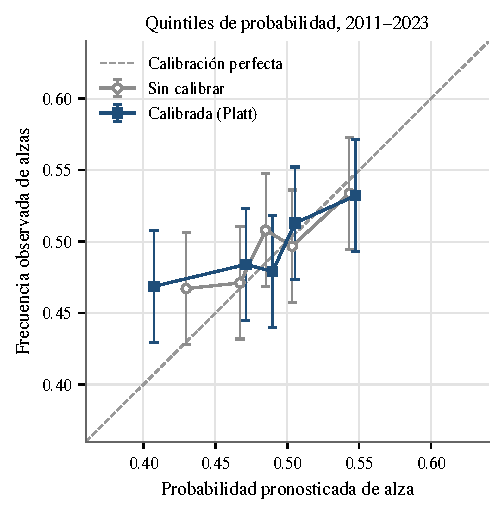
\includegraphics[width=0.55\textwidth]{fig2_confiabilidad.pdf}
\caption{Diagrama de confiabilidad, 2011--2023. Cada punto es un quintil de días ordenados por probabilidad pronosticada; las barras son intervalos de confianza al 95\%. La línea punteada es la calibración perfecta.}\label{fig:confiabilidad}
\end{figure}

\subsubsection{Valor económico}
La Tabla~\ref{tab:economico} presenta lo que importa a un inversionista: cuánto dinero gana la estrategia y con qué riesgo, frente a las referencias. En validación, la estrategia con M1 y \(c=\tfrac14\) gana 12,1\% anual neto de carry y costos, con una volatilidad de 13,1\% y un Sharpe de 0,92. Comprar dólares y mantenerlos ganó 0,4\% anual en el mismo período, con más volatilidad. La regla de exposición es selectiva: se abstiene el 54\% de los días y toma la exposición máxima solo el 3\% de las veces. Su pérdida máxima acumulada es de 10\%, frente a 35\% de comprar siempre.

\begin{table}[htbp]\centering\small
\caption{Valor económico de la estrategia y de las referencias}\label{tab:economico}
\begin{threeparttable}
\begin{tabular}{l rrrr rr rr}
\toprule
Estrategia & Ret.\ neto & Vol. & Sharpe & Pérd.\ máx. & \% en 0 & \% en $\pm3$ & DA act. & DA@3x \\
\midrule
\multicolumn{9}{l}{\emph{Panel A: validación, 2020--2023}} \\
M1, $c=\tfrac14$ & 12,08 & 13,08 & 0,92 & $-9{,}98$ & 54,3 & 3,3 & 55 & 52 \\
M1, $c=\tfrac15$ & 9,68 & 10,96 & 0,88 & $-8{,}24$ & 62,7 & 2,1 & 55 & 52 \\
Señal con tamaño fijo & 8,91 & 15,59 & 0,57 & $-37{,}77$ & 0,0 & 0,0 & 54 & --- \\
Comprar siempre ($+1$) & 0,38 & 15,60 & 0,02 & $-35{,}17$ & 0,0 & 0,0 & 49 & --- \\
Comprar siempre ($+3$) & 1,15 & 46,79 & 0,02 & $-105{,}52$ & 0,0 & 100,0 & 49 & 49 \\
No operar & 0,00 & 0,00 & --- & 0,00 & 100,0 & 0,0 & --- & --- \\
\midrule
\multicolumn{9}{l}{\emph{Panel B: fuera de muestra, 2011--2019}} \\
M1, $c=\tfrac14$ & 16,50 & 20,46 & 0,81 & $-33{,}99$ & 25,2 & 36,5 & 50 & 52 \\
M1, $c=\tfrac15$ & 18,42 & 19,48 & 0,95 & $-31{,}37$ & 29,7 & 31,3 & 51 & 53 \\
Señal con tamaño fijo & 6,39 & 10,18 & 0,63 & $-23{,}71$ & 0,0 & 0,0 & 52 & --- \\
Comprar siempre ($+1$) & 1,56 & 10,20 & 0,15 & $-26{,}95$ & 0,0 & 0,0 & 50 & --- \\
Comprar siempre ($+3$) & 4,69 & 30,60 & 0,15 & $-80{,}86$ & 0,0 & 100,0 & 50 & 50 \\
No operar & 0,00 & 0,00 & --- & 0,00 & 100,0 & 0,0 & --- & --- \\
\bottomrule
\end{tabular}
\begin{tablenotes}\footnotesize
\item \emph{Nota:} retorno neto anual y volatilidad anual en \%, netos de carry y de un costo de 2 pb por unidad de cambio de exposición. Pérdida máxima: mayor caída de la suma acumulada de retornos logarítmicos diarios, en puntos porcentuales (por eso puede superar 100). DA act.: acierto en los días con exposición distinta de cero (\%). 2010 se excluye porque su probabilidad no está calibrada.
\end{tablenotes}
\end{threeparttable}
\end{table}

La Figura~\ref{fig:curva} muestra la trayectoria completa, en el formato que piden las bases del torneo: el resultado acumulado neto de la estrategia frente a las referencias y, debajo, la exposición de cada día. En validación la estrategia sube de manera sostenida mientras comprar dólares termina cerca de cero, y la mayor parte del tiempo está sin posición o con exposición de uno.

\begin{figure}[htbp]\centering
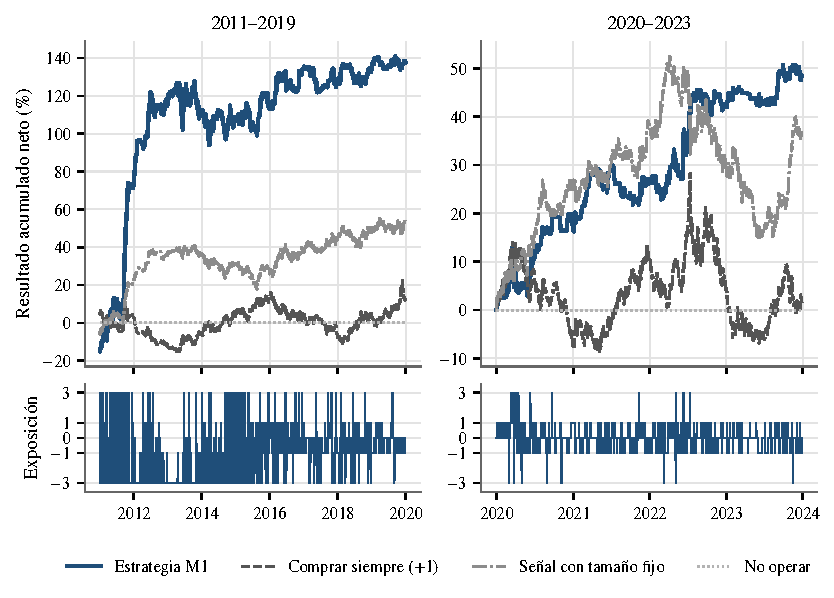
\includegraphics[width=\textwidth]{fig1_curva_resultado.pdf}
\caption{Resultado acumulado neto de carry y costos de la estrategia M1 ($c=\tfrac14$, 2 pb) y de las referencias (panel superior, suma de retornos logarítmicos diarios en \%), y exposición diaria de la estrategia (panel inferior).}\label{fig:curva}
\end{figure}

El tramo 2011--2019 muestra otra cara de la misma estrategia. Allí la volatilidad del peso era menor y la señal NY más fuerte (Sección~\ref{sec:datos}), de modo que la ventaja esperada era grande en relación con el riesgo y la regla tomó la exposición máxima el 36\% de los días. El retorno fue mayor, 16,5\% anual, pero también la pérdida máxima, de 34\%. El acierto en los días activos fue de solo 50\%, y aun así la estrategia ganó dinero: acertó en los días de mayor movimiento, el mismo patrón que \citet{gonzalez2026} documenta para el S\&P~500. Como se muestra en la Sección~\ref{sec:robustez}, ese resultado se concentra en 2011 y 2012, dos años con huecos en los datos. Con \(c=\tfrac15\) el resultado ajustado por riesgo mejora en 2011--2019 y empeora levemente en 2020--2023, por lo que ninguno de los dos valores domina y mantenemos el prerregistrado (\(c=\tfrac14\)).

\subsubsection{Evaluación formal frente a las referencias}
La Tabla~\ref{tab:formal} pasa de las magnitudes a la inferencia. En ambos tramos la estrategia gana más que no operar con significancia: en validación, la diferencia de 12,1 puntos porcentuales anuales tiene un intervalo de confianza de 1,9 a 22,7 y un p-valor de 0,012, que sobrevive a la corrección de Holm (0,049). Frente a comprar siempre la diferencia es de magnitud similar, 11,7 puntos al año, pero el intervalo incluye el cero y el p-valor es 0,082. Frente a comprar siempre con exposición 3 la diferencia es aun mayor en magnitud, pero esa referencia es tan volátil que no se puede distinguir de cero. La regla de exposición supera a la señal con tamaño fijo en 2011--2019 (\(p=0{,}048\)), pero no en 2020--2023, donde casi toda la ganancia proviene de acertar la dirección y no del tamaño.

\begin{table}[htbp]\centering\small
\caption{Evaluación formal: estrategia M1 ($c=\tfrac14$) frente a las referencias}\label{tab:formal}
\begin{threeparttable}
\begin{tabular}{l r c ccc rc}
\toprule
 & \multicolumn{5}{c}{Diferencia de retorno neto anual} & \multicolumn{2}{c}{Diferencia de Sharpe} \\
\cmidrule(lr){2-6}\cmidrule(lr){7-8}
Referencia & Dif. & IC 95\% & $p$ boot. & $p$ DM & $p$ Holm & Dif. & $p$ boot. \\
\midrule
\multicolumn{8}{l}{\emph{Panel A: validación, 2020--2023}} \\
No operar & 12,08 & [1,90; 22,65] & 0,012 & 0,012 & 0,049 & 0,92 & 0,014 \\
Comprar siempre ($+1$) & 11,70 & [$-4{,}74$; 28,20] & 0,082 & 0,090 & 0,246 & 0,90 & 0,073 \\
Comprar siempre ($+3$) & 10,93 & [$-32{,}63$; 54,93] & 0,304 & 0,317 & 0,608 & 0,90 & 0,073 \\
Señal con tamaño fijo & 3,17 & [$-12{,}30$; 19,56] & 0,330 & 0,337 & 0,608 & 0,35 & 0,264 \\
\midrule
\multicolumn{8}{l}{\emph{Panel B: fuera de muestra, 2011--2019}} \\
No operar & 16,50 & [1,02; 33,34] & 0,027 & 0,014 & 0,108 & 0,81 & 0,016 \\
Comprar siempre ($+1$) & 14,94 & [$-4{,}09$; 34,40] & 0,067 & 0,054 & 0,144 & 0,65 & 0,128 \\
Comprar siempre ($+3$) & 11,81 & [$-17{,}93$; 41,68] & 0,210 & 0,216 & 0,210 & 0,65 & 0,128 \\
Señal con tamaño fijo & 10,12 & [$-0{,}91$; 22,37] & 0,048 & 0,032 & 0,144 & 0,18 & 0,228 \\
\bottomrule
\end{tabular}
\begin{tablenotes}\footnotesize
\item \emph{Nota:} diferencias en puntos porcentuales anuales. Bootstrap estacionario pareado con 10.000 réplicas y bloques de 10 jornadas en promedio; intervalo de confianza por percentiles. Los p-valores son de una cola y no cambian sustancialmente con bloques de 5 o 20 jornadas. Holm se aplica sobre las cuatro comparaciones de cada panel.
\end{tablenotes}
\end{threeparttable}
\end{table}

Por último, el \emph{Deflated Sharpe Ratio} pone el Sharpe observado en perspectiva de las 48 variantes probadas. En 2011--2019 el Sharpe de 0,81 supera holgadamente el umbral de 0,45 que se esperaría obtener por azar entre esos ensayos, con una probabilidad de 0,85 de reflejar habilidad real. En 2020--2023 el umbral sube a 0,74, porque las variantes difieren más entre sí en ese tramo, y la probabilidad baja a 0,65. Ninguno de los dos alcanza el 0,95 habitual.

En síntesis, la validación respalda que la señal de Nueva York contiene información sobre la dirección del peso y que la estrategia gana dinero de manera significativa frente a no operar. La evidencia de que gana más que comprar dólares es económicamente grande, pero estadísticamente marginal, lo que es coherente con la baja potencia anticipada en la Sección~\ref{sec:evaluacion}.

\subsection{Prueba (2024 -- octubre 2026)}\label{sec:prueba}
\pendiente{Corrida única del 8 de noviembre. Se reporta tal como salga, con las mismas tablas de esta sección.}

% ---------- secciones/07_robustez ----------
\section{Robustez}\label{sec:robustez}

Esta sección somete los resultados de validación a cuatro preguntas que haría un operador antes de poner dinero en la estrategia: si depende de la fracción de Kelly elegida, si la ganancia está repartida en el tiempo o depende de pocos episodios, si es capturable cuando se opera a precios efectivamente disponibles y cuánto puede costar operar antes de que deje de ser rentable.

\subsection{Fracción de Kelly}
Con \(c=\tfrac15\) la estrategia apuesta un 20\% menos que con \(c=\tfrac14\). En validación gana 9,7\% anual con un Sharpe de 0,88, frente a 12,1\% y 0,92 de la regla principal, y en 2011--2019 gana 18,4\% con un Sharpe de 0,95, frente a 16,5\% y 0,81 (Tabla~\ref{tab:economico}). Ninguna de las dos fracciones domina a la otra en ambos tramos, y el costo de equilibrio es prácticamente el mismo (Figura~\ref{fig:costos}). Mantenemos la fracción prerregistrada.

\subsection{Estabilidad en el tiempo}
La Tabla~\ref{tab:anual} desagrega el resultado por año. En validación, la estrategia gana dinero en los cuatro años, entre 5,9\% y 16,8\%, mientras que comprar dólares pierde en tres de ellos. El resultado tampoco depende de unos pocos días: excluyendo el primer semestre de 2020, que incluye el inicio de la pandemia, el Sharpe de validación es 1,00, y eliminando los 10 mejores y los 10 peores días es 1,02. Un placebo que mantiene el tamaño de cada posición pero sortea su signo genera un Sharpe superior al observado solo en el 4\% de 1.000 sorteos.

\begin{table}[htbp]\centering\small
\caption{Resultado de la estrategia por año}\label{tab:anual}
\begin{threeparttable}
\begin{tabular}{l rr rr r}
\toprule
Año & Ret.\ neto (\%) & Sharpe & \% en 0 & \% en $\pm3$ & Comprar siempre (\%) \\
\midrule
2011\tnote{a} & 72,6 & 2,34 & 4,4 & 80,2 & 4,2 \\
2012\tnote{a} & 45,8 & 3,26 & 10,1 & 68,2 & $-16{,}6$ \\
2013 & $-6{,}7$ & $-0{,}26$ & 2,5 & 91,4 & 6,2 \\
2014 & $-3{,}5$ & $-0{,}17$ & 8,7 & 44,8 & 9,8 \\
2015 & 6,4 & 0,33 & 19,4 & 34,3 & 10,5 \\
2016 & 19,3 & 1,24 & 37,3 & 8,2 & $-10{,}0$ \\
2017 & $-5{,}5$ & $-0{,}53$ & 45,9 & 11,4 & $-11{,}8$ \\
2018 & 5,7 & 0,50 & 33,5 & 10,4 & 12,7 \\
2019 & 3,4 & 0,42 & 54,5 & 0,8 & 7,9 \\
\midrule
2020 & 16,8 & 0,95 & 47,2 & 9,9 & $-7{,}4$ \\
2021 & 10,3 & 1,16 & 55,0 & 0,4 & 18,2 \\
2022 & 15,4 & 1,02 & 51,4 & 2,4 & $-6{,}0$ \\
2023 & 5,9 & 0,71 & 63,4 & 0,4 & $-3{,}2$ \\
\bottomrule
\end{tabular}
\begin{tablenotes}\footnotesize
\item \emph{Nota:} M1 calibrado, \(c=\tfrac14\), costo de 2 pb. Retornos netos de carry, como suma de retornos logarítmicos diarios del año.
\item[a] Años con huecos en la serie del USD/CLP: 2012 tiene solo 140 jornadas y el 20\% de sus retornos abarca más de tres días corridos.
\end{tablenotes}
\end{threeparttable}
\end{table}

El tramo 2011--2019 es menos estable. Gana en 6 de 9 años, pero su resultado se concentra en 2011 y 2012, que suman un retorno anual promedio de 84\% con un Sharpe de 2,6. Entre 2013 y 2019 la estrategia gana solo 2,8\% anual, con un Sharpe de 0,16. Hay dos lecturas posibles y no podemos descartar ninguna. La primera es económica: 2011 fue el año con la correlación más alta entre la señal NY y el peso de toda la muestra (0,26), y la regla aprovechó esa ventaja con exposiciones grandes. La segunda es de datos: 2011 y 2012 son los años con huecos en la serie (Sección~\ref{sec:auditoria}), y en 2012 uno de cada cinco retornos abarca más de tres días corridos, lo que puede amplificar artificialmente las ganancias. En cualquier caso, la conclusión prudente es que el desempeño de 2011--2019 depende de dos años atípicos, y que la evidencia más confiable es la de validación, que es estable año a año.

\subsection{Ejecución a precios disponibles}
La convención del torneo liquida la exposición decidida al cierre de \(t\) con el precio de cierre de \(t+1\), como si se pudiera operar al mismo precio con que se decide. Un operador que decide al cierre local, en cambio, recién puede ejecutar a la apertura de la jornada siguiente. La Tabla~\ref{tab:ejecucion} separa el retorno de cada jornada en sus dos tramos y evalúa la misma secuencia de posiciones con distintos precios de ejecución.

\begin{table}[htbp]\centering\small
\caption{Resultado según el precio de ejecución}\label{tab:ejecucion}
\begin{threeparttable}
\begin{tabular}{l rr c rr}
\toprule
 & \multicolumn{2}{c}{2011--2019} & & \multicolumn{2}{c}{2020--2023} \\
\cmidrule{2-3}\cmidrule{5-6}
Tramo del retorno & Ret.\ neto (\%) & Sharpe & & Ret.\ neto (\%) & Sharpe \\
\midrule
Cierre a cierre (convención del torneo) & 16,5 & 0,81 & & 12,1 & 0,92 \\
Apertura a apertura (ejecución realista) & $-14{,}5$ & $-0{,}67$ & & 10,7 & 0,68 \\
\midrule
\multicolumn{6}{l}{\emph{Descomposición del retorno de \(t+1\)}} \\
Cierre de \(t\) a apertura de \(t+1\) (no transable) & 20,9 & 1,39 & & 7,3 & 0,76 \\
Apertura a cierre de \(t+1\) (sesión) & $-12{,}7$ & $-0{,}84$ & & 2,5 & 0,24 \\
\bottomrule
\end{tabular}
\begin{tablenotes}\footnotesize
\item \emph{Nota:} mismas posiciones en todas las filas (M1 calibrado, \(c=\tfrac14\)), costo de 2 pb. El carry se asigna al tramo cierre a cierre y apertura a apertura; los tramos de la descomposición no incluyen carry ni se suman exactamente.
\end{tablenotes}
\end{threeparttable}
\end{table}

El resultado es el más importante de esta sección para quien quiera ganar dinero con la estrategia. En 2011--2019 toda la ventaja está en el tramo entre el cierre local y la apertura del día siguiente, que no es transable: allí la estrategia obtiene un Sharpe de 1,39. Durante la sesión siguiente el peso revierte parte de ese movimiento, y quien ejecuta a la apertura pierde 14,5\% anual. En validación el panorama es mejor: con ejecución realista la estrategia gana 10,7\% anual con un Sharpe de 0,68, porque la ganancia se reparte entre el tramo nocturno y la sesión. Esto es consistente con el mecanismo de \emph{nonsynchronous trading} \citep{lo1990}: la señal anticipa el precio al que abrirá el peso, y la ventaja capturable depende de cuánto del ajuste ocurre después de la apertura. Un operador con acceso al mercado \emph{offshore} de forwards no entregables, que transa después del cierre local, podría capturar parte del tramo nocturno; evaluarlo requiere datos intradiarios que la base no contiene.


\begin{figure}[htbp]\centering
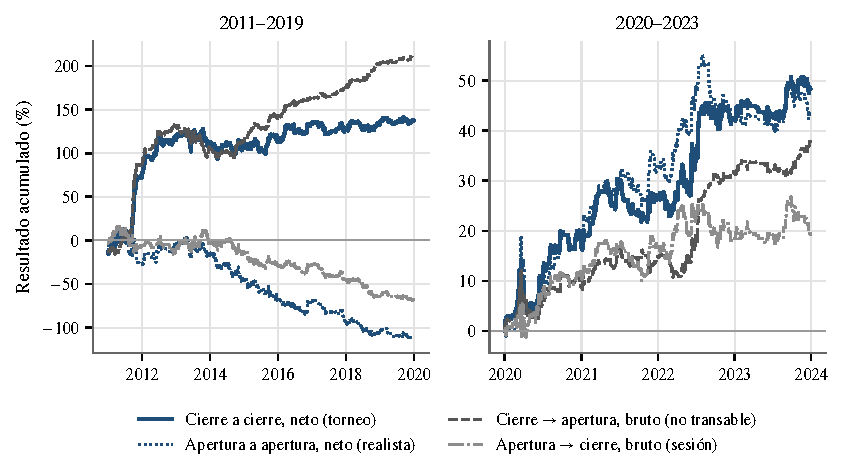
\includegraphics[width=\textwidth]{fig3_tramos_retorno.pdf}
\caption{Resultado acumulado de las mismas posiciones según el tramo del retorno de la jornada siguiente. ``Cierre a cierre'' es la convención del torneo; ``apertura a apertura'', la ejecución disponible para quien decide al cierre local.}\label{fig:tramos}
\end{figure}

La Figura~\ref{fig:tramos} muestra la misma descomposición en el tiempo. En 2011--2019 la ganancia del tramo nocturno crece casi todos los años mientras la de la sesión cae de forma persistente, de modo que quien opera a la apertura pierde de manera sistemática. En 2020--2023 ambos tramos ganan, y la ejecución realista sigue de cerca a la convención del torneo.

\subsection{Costos de transacción}
El costo base de 2 puntos base por unidad de cambio de exposición corresponde a un operador institucional. Para un inversionista minorista el costo es mayor y depende del canal. La Tabla~\ref{tab:canales} resume los spreads observados el 20 de octubre de 2026, con un tipo de cambio de referencia de unos 985 pesos, en que un peso de spread equivale a unos 10 puntos base. El costo por unidad de cambio es aproximadamente la mitad del spread, porque cada operación cruza medio spread.

\begin{table}[htbp]\centering\small
\caption{Costo de operar USD/CLP para un inversionista minorista}\label{tab:canales}
\begin{threeparttable}
\begin{tabular}{l r r c}
\toprule
Canal & Spread (CLP) & Costo (pb) & Venta corta \\
\midrule
CFD con \emph{broker} internacional & 0,4--0,8 & 2--4\tnote{a} & Sí \\
Plataforma de criptoactivos (USDT/USDC) & 1,5--2,0 & 7--10 & No \\
Aplicaciones y corredoras en línea & 2--8 & 10--40 & No \\
Fondo en dólares (Fintual) & 9,2 & 47 & No \\
Casa de cambio (AFEX) & 20 & 100 & No \\
Banca tradicional & 15--50 & 75--250 & No \\
Banca privada, alto patrimonio\tnote{b} & 3 por operación & 30 & Según mandato \\
\bottomrule
\end{tabular}
\begin{tablenotes}\footnotesize
\item \emph{Fuentes:} \citet{dolaronline2026}, \citet{admiral2026} y \citet{rankia2026}. Costo por unidad de cambio de exposición: medio spread dividido por un tipo de cambio de 985. Venta corta: si el canal permite apostar a la baja del dólar; solo el CFD permite además exposiciones apalancadas.
\item[a] Más un cargo diario de financiamiento (\emph{swap}) de alrededor de 0,04\% de la posición, tanto comprada como vendida.
\item[b] Recargo sobre el precio de mercado en cada compra o venta de dólares en carteras discrecionales de alto patrimonio, según la experiencia profesional de uno de los autores; varía según la importancia del cliente.
\end{tablenotes}
\end{threeparttable}
\end{table}

La Figura~\ref{fig:costos} responde dónde deja de ser rentable la estrategia: muestra cómo cae su retorno neto a medida que sube el costo por unidad de cambio de exposición, manteniendo las posiciones decididas con el costo del torneo, y ubica debajo el rango de costos de cada canal. La estrategia rota mucho: cambia en promedio 225 unidades de exposición al año en 2011--2019 y 113 en 2020--2023, por lo que cada punto base adicional le resta entre 1,1 y 2,3 puntos porcentuales de retorno anual. El retorno neto se hace cero con un costo de 12,7 puntos base en validación y de 9,3 en 2011--2019. Con \(c=\tfrac15\) esos umbrales son 12,1 y 10,9 puntos base; con ejecución a la apertura, 11,5 en validación, mientras que en 2011--2019 la estrategia pierde dinero antes de costos.

\begin{figure}[htbp]\centering
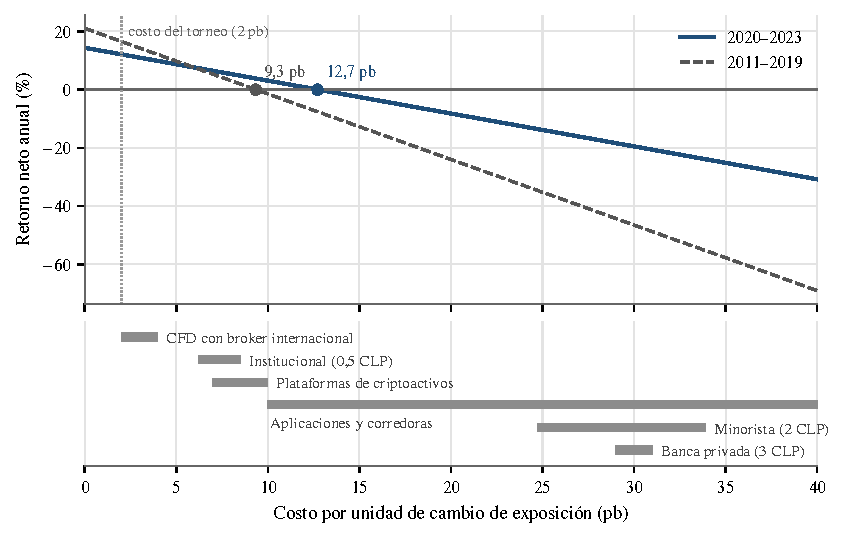
\includegraphics[width=\textwidth]{fig4_costos.pdf}
\caption{Retorno neto anual de la estrategia según el costo por unidad de cambio de exposición (posiciones decididas con 2 pb, convención cierre a cierre). Los puntos marcan el costo de equilibrio. Abajo, el rango de costo de cada canal (Tabla~\ref{tab:canales} y Sección~\ref{sec:robustez}); casas de cambio y banca tradicional cuestan más de 75 pb y quedan fuera del gráfico.}\label{fig:costos}
\end{figure}

Si la regla de exposición conoce el costo verdadero y decide en consecuencia, tampoco rescata la estrategia: cuando el costo sube, simplemente deja de operar, y su Sharpe cae a 0,1--0,2, porque la señal es de horizonte diario y no sobrevive a operar con poca frecuencia.

Con un costo de equilibrio de 9 a 13 puntos base, la estrategia solo es rentable en el canal más barato: un CFD con un \emph{broker} internacional, que además es el único que permite vender dólares en corto y tomar exposiciones de 3. Las plataformas de criptoactivos quedan cerca del equilibrio y no permiten posiciones cortas; todos los demás canales minoristas harían perder dinero. Incluso en el CFD hay un costo adicional: el cargo diario de financiamiento, de unos 13--15\% anual sobre la posición, supera con creces el diferencial de tasas que ya descuenta el retorno en exceso. Con el costo de un CFD (2 a 4 puntos base) y un sobrecosto de financiamiento de 13\% anual, la estrategia gana entre 3,0\% y 5,3\% anual en validación, con un Sharpe de 0,23 a 0,41, y pierde dinero en 2011--2019.

\subsection{Perfiles de inversionista}
Para resumir la discusión de costos en un resultado concreto, definimos dos perfiles a partir de la experiencia profesional de uno de los autores en carteras discrecionales de alto patrimonio: un \textbf{inversionista institucional}, que paga 0,5 pesos por dólar comprado o vendido, y un \textbf{inversionista minorista}, que paga 2 pesos. Como el costo está en pesos, en términos porcentuales es mayor cuando el dólar está más barato: el costo institucional equivale en promedio a 8,5 puntos base en 2011--2019, con un tipo de cambio cercano a 600 pesos, y a 6,2 en 2020--2023, con uno cercano a 820; el minorista, a 34 y 25 puntos base. Cada perfil decide con la regla de exposición usando su propio costo, como lo haría un inversionista que sabe cuánto le cobran. Como comparación, la Tabla~\ref{tab:perfiles} muestra también qué le ocurriría a cada uno si replicara las posiciones decididas con el costo del torneo. Los perfiles se fijaron el 21 de octubre, antes de la corrida en el tramo de prueba, y se reportarán junto con el resultado oficial.

\begin{table}[htbp]\centering\small
\caption{Resultado por perfil de inversionista}\label{tab:perfiles}
\begin{threeparttable}
\begin{tabular}{l r rrrr}
\toprule
Perfil y regla & Costo (pb) & Ret.\ neto & Sharpe & Pérd.\ máx. & \% en 0 \\
\midrule
\multicolumn{6}{l}{\emph{Panel A: validación, 2020--2023}} \\
Torneo, regla oficial & 2,0 & 12,08 & 0,92 & $-9{,}98$ & 54,3 \\
Institucional, regla propia & 6,2 & 2,00 & 0,17 & $-16{,}77$ & 51,7 \\
Institucional, posiciones del torneo & 6,2 & 7,51 & 0,57 & $-11{,}86$ & 54,3 \\
Minorista, regla propia & 24,7 & 0,00 & --- & 0,00 & 100,0 \\
Minorista, posiciones del torneo & 24,7 & $-12{,}97$ & $-0{,}97$ & $-60{,}03$ & 54,3 \\
\midrule
\multicolumn{6}{l}{\emph{Panel B: fuera de muestra, 2011--2019}} \\
Torneo, regla oficial & 2,0 & 16,50 & 0,81 & $-33{,}99$ & 25,2 \\
Institucional, regla propia & 8,5 & 7,04 & 0,45 & $-32{,}71$ & 33,1 \\
Institucional, posiciones del torneo & 8,5 & 1,00 & 0,05 & $-70{,}21$ & 25,2 \\
Minorista, regla propia & 33,9 & $-0{,}65$ & $-0{,}29$ & $-5{,}43$ & 99,4 \\
Minorista, posiciones del torneo & 33,9 & $-59{,}02$ & $-2{,}69$ & $-478{,}90$ & 25,2 \\
\bottomrule
\end{tabular}
\begin{tablenotes}\footnotesize
\item \emph{Nota:} institucional, 0,5 pesos por dólar transado; minorista, 2 pesos. Costo: promedio del período en puntos base (pesos divididos por el tipo de cambio de cada día). Retorno neto anual y pérdida máxima en \%, netos de carry. ``Regla propia'': la ecuación~\eqref{eq:kelly} con el costo del perfil. ``Posiciones del torneo'': las posiciones decididas con 2 pb, cobrando el costo del perfil.
\end{tablenotes}
\end{threeparttable}
\end{table}

El inversionista institucional gana dinero en ambos tramos, pero bastante menos que bajo la convención del torneo: entre 2,0\% y 7,5\% anual en validación, según la regla, con un Sharpe de 0,17 a 0,57. El minorista, sabiendo su costo, prácticamente no opera, y su resultado es equivalente a no operar; si replicara las posiciones del torneo perdería 13\% anual en validación. La tabla también muestra un resultado poco intuitivo: en validación, al institucional le habría convenido mantener las posiciones decididas con un costo menor que el suyo, porque la regla que conoce su costo opera menos y deja pasar días con ganancias. Esto confirma que la ventaja de la señal es de alta frecuencia: reducir la rotación para ahorrar costos también reduce la ganancia, casi en la misma proporción.

\subsection{Síntesis}
La estrategia es robusta en validación: gana en todos los años, no depende de pocos días ni de la fracción de Kelly, y su ventaja no se explica por azar. Sus límites son tres. El desempeño de 2011--2019 depende de dos años atípicos con huecos en los datos. Una parte de la ventaja ocurre fuera del horario en que se puede operar en Chile. Y la rentabilidad solo sobrevive a costos institucionales: un inversionista institucional gana entre 2\% y 7,5\% anual en validación, y un minorista, en cualquier canal, gana poco o nada. Para una mesa de dinero con costos bajos y acceso al mercado \emph{offshore}, la estrategia tiene valor; para un inversionista minorista que opera en Chile durante el horario local, prácticamente no.

% ---------- secciones/08_monitoreo ----------
\section{Monitoreo en vivo}\label{sec:monitoreo}
\pendiente{Procedimiento diario (\texttt{run\_daily.py}), registro de señales y resultados del 13 de noviembre al 1 de diciembre.}


% ---------- secciones/09_conclusiones ----------
\section{Conclusiones}\label{sec:conclusiones}
\pendiente{Respuesta a la pregunta, límites (potencia, asincronía, costos retail) y extensiones.}


\newpage
\renewcommand{\refname}{Referencias}
% Referencias incluidas en el mismo archivo (generadas desde referencias.bib con estilo apalike-es)
\begin{thebibliography}{}

\bibitem[{Admiral Markets}, 2026]{admiral2026}
{Admiral Markets} (2026).
\newblock Especificaciones del contrato {USDCLP} ({CFD}).
\newblock \url{https://admiralmarkets.com/es/instrument/us-dollar-vs-chilean-peso-usdclp}. Consultado el 20 de octubre de 2026.

\bibitem[Bailey et~al., 2017]{bailey2017}
Bailey, D.~H., Borwein, J.~M., López~de Prado, M., y Zhu, Q.~J. (2017).
\newblock The probability of backtest overfitting.
\newblock {\em Journal of Computational Finance}, 20(4):39--69.

\bibitem[Bailey y López~de Prado, 2014]{bailey2014}
Bailey, D.~H. y López~de Prado, M. (2014).
\newblock The deflated {S}harpe ratio: Correcting for selection bias, backtest
  overfitting, and non-normality.
\newblock {\em Journal of Portfolio Management}, 40(5):94--107.

\bibitem[{Banco Central de Chile}, 2026]{ipom2026}
{Banco Central de Chile} (2026).
\newblock Informe de política monetaria, septiembre 2026.
\newblock Informe, Banco Central de Chile.

\bibitem[Brunnermeier et~al., 2009]{brunnermeier2008}
Brunnermeier, M.~K., Nagel, S., y Pedersen, L.~H. (2009).
\newblock Carry trades and currency crashes.
\newblock En {\em NBER Macroeconomics Annual 2008}, vol.~23, pp. 313--347.
  University of Chicago Press.

\bibitem[Burnside et~al., 2011]{burnside2011}
Burnside, C., Eichenbaum, M., Kleshchelski, I., y Rebelo, S. (2011).
\newblock Do peso problems explain the returns to the carry trade?
\newblock {\em Review of Financial Studies}, 24(3):853--891.

\bibitem[Chen y Rogoff, 2003]{chen2003}
Chen, Y.-c. y Rogoff, K. (2003).
\newblock Commodity currencies.
\newblock {\em Journal of International Economics}, 60(1):133--160.

\bibitem[Chen et~al., 2010]{chen2010}
Chen, Y.-c., Rogoff, K.~S., y Rossi, B. (2010).
\newblock Can exchange rates forecast commodity prices?
\newblock {\em Quarterly Journal of Economics}, 125(3):1145--1194.

\bibitem[Clark y West, 2007]{clark2007}
Clark, T.~E. y West, K.~D. (2007).
\newblock Approximately normal tests for equal predictive accuracy in nested
  models.
\newblock {\em Journal of Econometrics}, 138(1):291--311.

\bibitem[De~Gregorio, 2009]{degregorio2009}
De~Gregorio, J. (2009).
\newblock El crecimiento en {C}hile y el cobre.
\newblock Presentación en la Conferencia CESCO 25 años, Banco Central de Chile, septiembre de 2009.

\bibitem[Diebold y Mariano, 1995]{diebold1995}
Diebold, F.~X. y Mariano, R.~S. (1995).
\newblock Comparing predictive accuracy.
\newblock {\em Journal of Business \& Economic Statistics}, 13(3):253--263.

\bibitem[{Dólar Online}, 2026]{dolaronline2026}
{Dólar Online} (2026).
\newblock Comparador del dólar en {C}hile.
\newblock \url{https://www.dolaronline.cl/comparador-dolar-chile/}. Consultado el 20 de octubre de 2026.

\bibitem[Evans y Lyons, 2002]{evans2002}
Evans, M. D.~D. y Lyons, R.~K. (2002).
\newblock Order flow and exchange rate dynamics.
\newblock {\em Journal of Political Economy}, 110(1):170--180.

\bibitem[González~Cañón, 2026]{gonzalez2026}
González~Cañón, D. (2026).
\newblock Explorando los límites de la eficiencia del mercado: enfoques
  clásicos y contemporáneos de modelado cuantitativo para la predicción
  direccional y generación de alfa en el {S\&P} 500.
\newblock Tesis de Magíster en Finanzas, Facultad de Economía y Negocios, Universidad de
  Chile.

\bibitem[Harvey et~al., 1997]{harvey1997}
Harvey, D., Leybourne, S., y Newbold, P. (1997).
\newblock Testing the equality of prediction mean squared errors.
\newblock {\em International Journal of Forecasting}, 13(2):281--291.

\bibitem[Holm, 1979]{holm1979}
Holm, S. (1979).
\newblock A simple sequentially rejective multiple test procedure.
\newblock {\em Scandinavian Journal of Statistics}, 6(2):65--70.

\bibitem[Jaramillo y Selaive, 2006]{jaramillo2006}
Jaramillo, P. y Selaive, J. (2006).
\newblock Actividad especulativa y precio del cobre.
\newblock Documento de Trabajo 384, Banco Central de Chile.

\bibitem[Kelly, 1956]{kelly1956}
Kelly, John~L., J. (1956).
\newblock A new interpretation of information rate.
\newblock {\em Bell System Technical Journal}, 35(4):917--926.

\bibitem[Lo y MacKinlay, 1990]{lo1990}
Lo, A.~W. y MacKinlay, A.~C. (1990).
\newblock An econometric analysis of nonsynchronous trading.
\newblock {\em Journal of Econometrics}, 45(1--2):181--211.

\bibitem[Lustig et~al., 2011]{lustig2011}
Lustig, H., Roussanov, N., y Verdelhan, A. (2011).
\newblock Common risk factors in currency markets.
\newblock {\em Review of Financial Studies}, 24(11):3731--3777.

\bibitem[Lustig y Verdelhan, 2008]{lustig2008}
Lustig, H. y Verdelhan, A. (2008).
\newblock The cross-section of foreign currency risk premia and consumption
  growth risk: A reply.
\newblock NBER Working Paper 13812, National Bureau of Economic Research.

\bibitem[Meese y Rogoff, 1983]{meese1983}
Meese, R.~A. y Rogoff, K. (1983).
\newblock Empirical exchange rate models of the seventies: Do they fit out of
  sample?
\newblock {\em Journal of International Economics}, 14(1--2):3--24.

\bibitem[Menkhoff et~al., 2012]{menkhoff2012}
Menkhoff, L., Sarno, L., Schmeling, M., y Schrimpf, A. (2012).
\newblock Currency momentum strategies.
\newblock {\em Journal of Financial Economics}, 106(3):660--684.

\bibitem[Newey y West, 1987]{newey1987}
Newey, W.~K. y West, K.~D. (1987).
\newblock A simple, positive semi-definite, heteroskedasticity and
  autocorrelation consistent covariance matrix.
\newblock {\em Econometrica}, 55(3):703--708.

\bibitem[Niculescu-Mizil y Caruana, 2005]{niculescu2005}
Niculescu-Mizil, A. y Caruana, R. (2005).
\newblock Predicting good probabilities with supervised learning.
\newblock En {\em Proceedings of the 22nd International Conference on Machine
  Learning}, pages 625--632.

\bibitem[Pesaran y Timmermann, 1992]{pesaran1992}
Pesaran, M.~H. y Timmermann, A. (1992).
\newblock A simple nonparametric test of predictive performance.
\newblock {\em Journal of Business \& Economic Statistics}, 10(4):461--465.

\bibitem[Platt, 1999]{platt1999}
Platt, J.~C. (1999).
\newblock Probabilistic outputs for support vector machines and comparisons to
  regularized likelihood methods.
\newblock En Smola, A.~J., Bartlett, P., Schölkopf, B., y Schuurmans, D.,
  editores, {\em Advances in Large Margin Classifiers}, pp. 61--74. MIT Press.

\bibitem[Politis y Romano, 1994]{politis1994}
Politis, D.~N. y Romano, J.~P. (1994).
\newblock The stationary bootstrap.
\newblock {\em Journal of the American Statistical Association},
  89(428):1303--1313.

\bibitem[{Rankia}, 2026]{rankia2026}
{Rankia} (2026).
\newblock Dónde comprar dólares en {C}hile: bancos vs. brokers online.
\newblock \url{https://www.rankia.cl/blog/como-invertir-forex/7188549-donde-comprar-dolares-chile-bancos-vs-brokers-online}. Publicado el 9 de febrero de 2026; consultado el 20 de octubre de 2026.

\bibitem[Rossi, 2013]{rossi2013}
Rossi, B. (2013).
\newblock Exchange rate predictability.
\newblock {\em Journal of Economic Literature}, 51(4):1063--1119.

\bibitem[Scholes y Williams, 1977]{scholes1977}
Scholes, M. y Williams, J. (1977).
\newblock Estimating betas from nonsynchronous data.
\newblock {\em Journal of Financial Economics}, 5(3):309--327.

\bibitem[White, 2000]{white2000}
White, H. (2000).
\newblock A reality check for data snooping.
\newblock {\em Econometrica}, 68(5):1097--1126.

\end{thebibliography}

\newpage
\appendix

% ---------- secciones/A_apendice ----------
\section{Registro de experimentos}\label{app:registro}

La Tabla~\ref{tab:registro} lista, en orden cronológico, cada análisis que miró datos durante el estudio, con la decisión que se tomó a partir de él. El registro se llevó desde el primer día en el archivo \texttt{reports/}\allowbreak\texttt{registro\_experimentos.csv} del repositorio, y en él se basa el número de ensayos del \emph{Deflated Sharpe Ratio}. Dos entradas (E10 y E12) se escribieron antes de correr el análisis que describen, como prerregistro.

\begin{table}[htbp]\centering\scriptsize
\caption{Registro de experimentos}\label{tab:registro}
\begin{tabularx}{\textwidth}{@{}l l >{\raggedright\arraybackslash}X >{\raggedright\arraybackslash}X >{\raggedright\arraybackslash}X@{}}
\toprule
ID & Fecha & Qué se probó & Resultado & Decisión \\
\midrule
E01 & 13 oct & Auditoría: correlación de 21 series del día \(t\) con el USD/CLP de \(t+1\), 2004--2023 & Solo las series que cierran en Nueva York anticipan el día siguiente & Señal NY al núcleo del modelo \\
E02 & 13 oct & Regla simple: signo de la señal NY, 2016--2023 & Sharpe 0,89 y 0,67 con costo de 2 pb & Exploratoria; no es el modelo \\
E03 & 13 oct & Escalera M0/M1/M2 con ventanas expansiva, móvil, promedio y calibrada, 2010--2023 & Clark-West: M1 supera a M0 (\(p=0{,}029\)); M2 no supera a M1 (\(p=0{,}68\)) & Modelo operativo: M1 \\
E04 & 13 oct & Regla prerregistrada: Kelly redondeado con filtro de costo, \(c=\tfrac14\) y \(\tfrac15\) & 87\% de los días en \(\pm3\) en 2011--2019; pérdida máxima de 71\% & Defecto de diseño: el redondeo ignora el riesgo \\
E05 & 13 oct & Kelly discreto por utilidad (ecuación~\ref{eq:kelly}), 2011--2023 & Sharpe 0,81 y 0,92; 54\% de días sin posición en 2020--2023 & Regla oficial desde el 13 de octubre \\
E06 & 13 oct & Robustez: por año, sin el primer semestre de 2020, recorte simétrico, placebo & Positivo los 4 años de validación; placebo \(p=0{,}040\) & Se mantiene la regla \\
E07 & 20 oct & Ejecución a la apertura frente a la convención del torneo, 2011--2023 & Apertura a apertura: Sharpe $-0{,}67$ y 0,68; tramo nocturno 1,39 y 0,76 & La ventaja vive en el tramo no transable; se reporta \\
E08 & 20 oct & Sensibilidad al costo (0--100 pb) y costo de equilibrio & Equilibrio de 9,3 y 12,7 pb; reoptimizar no rescata la estrategia & Costo oficial de 2 pb; canales minoristas en robustez \\
E09 & 20 oct & Evaluación formal frente a las referencias (diseño fijado antes de verla) & Frente a no operar \(p=0{,}012\); frente a comprar siempre \(p=0{,}082\) & No es una estrategia nueva \\
E10 & 20 oct & \emph{Prerregistro}: M1 + cobre COMEX; entra si Clark-West frente a M1 da \(p<0{,}05\) & \(p=0{,}551\) en validación; coeficiente del cobre \(t=0{,}47\) & Descartado; M1 sigue operativo \\
E11 & 20 oct & Diagnóstico por año de la estrategia & 2011--2012 concentran el resultado de 2011--2019, con huecos de datos & Se reporta en robustez \\
E12 & 21 oct & \emph{Prerregistro}: perfiles institucional (0,5 pesos) y minorista (2 pesos) & Institucional 2,0--7,5\% anual en validación; minorista no opera & Se reportan junto al resultado oficial \\
\bottomrule
\end{tabularx}
\begin{tablenotes}\footnotesize
\item \emph{Nota:} cuando hay dos cifras, corresponden a 2011--2019 y 2020--2023, respectivamente.
\end{tablenotes}
\end{table}

\paragraph{Número de ensayos.} El \emph{Deflated Sharpe Ratio} cuenta como ensayo cada variante cuyo resultado económico se observó antes de elegir la estrategia final: tres modelos (M1, M2 y M1C), cuatro versiones de cada uno (ventana expansiva, móvil, promedio y promedio calibrado), dos fracciones de Kelly (\(\tfrac14\) y \(\tfrac15\)) y dos reglas de exposición (la original y la de utilidad), en total \(N=48\). Los análisis de robustez, diagnóstico y evaluación (E06--E09, E11 y E12) no se cuentan como ensayos, porque no generaron estrategias candidatas: aplican la misma estrategia a otros precios, costos o subperíodos.

\section{Reproducibilidad}\label{app:repro}

Todo el análisis se reproduce con el código del repositorio y la base entregada por el laboratorio, sin otros datos ni pasos manuales.

\paragraph{Estructura del repositorio.}
\begin{itemize}\itemsep1pt
\item \texttt{src/config.py}: parámetros prerregistrados (muestra, variables, modelos, regla de exposición, costos y perfiles).
\item \texttt{src/datos.py}: lectura de la base y construcción de la tabla de variables, con una prueba automática de que ninguna variable usa información futura.
\item \texttt{src/modelo.py}: estimación \emph{walk-forward} del logit con ventanas expansiva y móvil, y calibración de Platt.
\item \texttt{src/evaluacion.py}: métricas, tests (Clark-West, Diebold-Mariano, Pesaran-Timmermann), regla de exposición, backtest, bootstrap estacionario, corrección de Holm y \emph{Deflated Sharpe Ratio}.
\item \texttt{src/auditoria.py}: auditoría de la base (Sección~\ref{sec:auditoria}).
\item \texttt{notebooks/01\_modelo\_nucleo.ipynb}: todos los resultados del informe, en 14 secciones.
\item \texttt{run\_daily.py}: señal diaria para el monitoreo en vivo.
\item \texttt{tests/test\_run\_daily.py}: verifica que la señal diaria reproduce exactamente el backtest.
\item \texttt{reports/registro\_experimentos.csv}: el registro de la Tabla~\ref{tab:registro}.
\end{itemize}

\paragraph{Cómo reproducir los resultados.} Con Python 3.11 o superior: (1) dejar el Excel de la base en la carpeta \texttt{data/}; (2) instalar las dependencias con \texttt{pip install -r requirements.txt}; (3) ejecutar el notebook completo, lo que toma uno a dos minutos. La Tabla~\ref{tab:origen} indica de qué sección del notebook sale cada tabla y figura del informe; las figuras se guardan en \texttt{reports/figuras/}. Las semillas del bootstrap y del placebo están fijas, por lo que los resultados son idénticos en cada ejecución.

\begin{table}[htbp]\centering\small
\caption{Origen de cada tabla y figura del informe}\label{tab:origen}
\begin{tabular}{l l}
\toprule
Tabla o figura & Sección del notebook \\
\midrule
\ref{tab:tramos} (tramos) y \ref{tab:series} (series) & Configuración (\texttt{src/config.py}) y diccionario de la base \\
\ref{tab:descriptivas} (estadísticas descriptivas) & 13 \\
\ref{tab:coef} (coeficientes) & 2 (M1, M2) y 11 (M1C) \\
\ref{tab:pronostico} y \ref{tab:tests} (pronóstico y tests) & 3, 4 y 11 \\
\ref{tab:economico} (valor económico) & 6 (panel A) y 13 (panel B) \\
\ref{tab:formal} (evaluación formal) & 10 \\
\ref{tab:anual} (resultado por año) & 7 y 13 \\
\ref{tab:ejecucion} (ejecución) & 8 \\
\ref{tab:canales} (canales minoristas) & Fuentes externas citadas en la tabla \\
Figura \ref{fig:costos} (costos) & 9 y 14 \\
\ref{tab:perfiles} (perfiles de inversionista) & 12 \\
Figuras \ref{fig:confiabilidad}, \ref{fig:curva} y \ref{fig:tramos} & 14 (\texttt{src/figuras.py}) \\
\bottomrule
\end{tabular}
\end{table}

\paragraph{Señal diaria.} Durante el monitoreo en vivo, \texttt{run\_daily.py} calcula la exposición de la jornada siguiente con el modelo congelado, siguiendo exactamente el procedimiento del backtest, y la anota en \texttt{reports/senales\_diarias.csv} junto con una huella del código con que se emitió. La huella permite verificar que el modelo no cambió durante el torneo. Antes de la fecha de congelamiento, el script rechaza fechas posteriores a 2023, para impedir que se examine el tramo de prueba por accidente.

\end{document}
